% PEPFAR and Growth: DiD and event studies for the economic outcomes
% Compile this file from inside tables/ (e.g. upload crown_results.tex together with
% the crown_did/ and crown_event_studies/ folders to Overleaf). Every table and
% figure it pulls in is generated by:
%   analysis/replication/did_econ.R
%   analysis/parallel_trends/event_study_econ_adjusted.R
\documentclass[11pt]{article}
\usepackage[margin=1in]{geometry}
\usepackage{amsmath}
\usepackage{booktabs}
\usepackage{graphicx}
\usepackage[hidelinks]{hyperref}

\title{PEPFAR and Growth: Difference-in-Differences and Event Studies\\for the Economic Outcomes}
\author{Anthony Babu\\Charles River Economics Lab}
\date{\today}

\begin{document}
\maketitle

\section*{Data and samples}

Country--year panel \texttt{pepfar\_panel\_1990\_2022\_FIXED.csv}, 1990--2022. Treatment
groups: all PEPFAR recipients (90 countries) and the 31 COP countries, each compared with
the 64 comparison countries valid through 2022 (\texttt{grp\_control\_kates}: Crown's 67
minus Venezuela, Colombia and Panama). Outcomes: the five in Crown et al.\ (2023) (GDP per
capita growth, female and male employment, girls' and boys' primary disengagement) and
three additions (GDP growth, log GDP per capita, log GDP). Adjusted models use the 11
baseline (2003) covariates of Crown et al.\ (2023) Table~1; countries missing any of them
drop out, which is why adjusted samples have about 100 (All PEPFAR) and 55 (COP) countries.
Standard errors are clustered by country throughout.

\section{Difference-in-differences}

Panel A of Tables~\ref{tab:did_all_pepfar}--\ref{tab:did_cop} is the specification of Crown
et al.\ (2023), pooled OLS with no fixed effects:
\begin{equation*}
Y_{it} = \beta_0 + \beta_1\,\text{Post}_t + \beta_2\,\text{PEPFAR}_i
       + \beta_3\,(\text{PEPFAR}_i \times \text{Post}_t) + \delta' X_i + \varepsilon_{it},
\end{equation*}
where $\text{Post}_t = 1$ from 2004 and $X_i$ are the baseline covariates. Panel B adds
country and year fixed effects and lets each baseline covariate have its own effect in
every year:
\begin{equation*}
Y_{it} = \alpha_i + \gamma_t + \beta\,(\text{PEPFAR}_i \times \text{Post}_t)
       + X_i' \delta_t + \varepsilon_{it}.
\end{equation*}
$\beta_3$ and $\beta$ are the difference-in-differences estimates.

\begin{table}[htbp]
\centering
\caption{Difference-in-differences, adjusted: All PEPFAR and COP}
\label{tab:did_combined}
\begin{tabular}{lcccc}
\toprule
 & \multicolumn{2}{c}{All PEPFAR vs.\ controls} & \multicolumn{2}{c}{COP vs.\ controls} \\
\cmidrule(lr){2-3}\cmidrule(lr){4-5}
 & Pooled OLS & TWFE & Pooled OLS & TWFE \\
 & (1) & (2) & (3) & (4) \\
\midrule
GDP pc growth & $2.509^{***}$ & $3.267^{*}$ & $2.615^{**}$ & $7.274$ \\
 & (0.906) & (1.673) & (0.995) & (4.636) \\
Female emp. & $-3.246^{***}$ & $0.284$ & $-4.148^{***}$ & $0.176$ \\
 & (1.119) & (1.486) & (1.351) & (2.382) \\
Male emp. & $0.346$ & $1.402$ & $-0.050$ & $2.322$ \\
 & (0.905) & (1.228) & (1.095) & (2.144) \\
Girls' diseng. & $-10.927^{***}$ & $1.730$ & $-10.753^{**}$ & $1.632$ \\
 & (3.290) & (4.421) & (4.505) & (8.093) \\
Boys' diseng. & $-9.934^{***}$ & $-0.921$ & $-12.282^{***}$ & $-5.110$ \\
 & (2.638) & (4.483) & (3.793) & (7.912) \\
GDP growth & $2.856^{***}$ & $3.567^{*}$ & $2.890^{***}$ & $7.402$ \\
 & (0.955) & (1.802) & (1.041) & (5.049) \\
log GDP pc & $0.069$ & $-0.003$ & $0.121$ & $-0.117$ \\
 & (0.095) & (0.167) & (0.124) & (0.450) \\
log GDP & $0.158$ & $-0.075$ & $0.219$ & $-0.237$ \\
 & (0.108) & (0.176) & (0.133) & (0.484) \\
\midrule
Countries (range across outcomes) & 98--104 & 96--104 & 53--58 & 53--58 \\
\bottomrule
\end{tabular}
\par\vspace{4pt}
\begin{minipage}{\textwidth}\footnotesize Each cell is the DiD coefficient (treatment group $\times$ Post) from a separate regression; full results in Tables~\ref{tab:did_all_pepfar} and~\ref{tab:did_cop}. Standard errors clustered by country in parentheses. Post $= 1$ for 2004 onward for every country. Sample 1990--2022; controls are the 64 comparison countries valid through 2022 (\texttt{grp\_control\_kates}). All models include the 11 baseline (2003) covariates of Crown et al.\ (2023) Table~1: GDP per capita, population, life expectancy, fertility, urban share, gross secondary enrollment, HIV prevalence, non-PEPFAR donor health aid per capita, domestic health expenditure per capita, US HIV aid before 2004, and World Bank income group. Pooled OLS enters them directly (no fixed effects). TWFE has country and year fixed effects and lets each covariate have its own coefficient in every year (income group enters as income group $\times$ year fixed effects). Disengagement is in percentage points. $^{*}p<0.10$, $^{**}p<0.05$, $^{***}p<0.01$.\end{minipage}
\end{table}

\begin{table}[htbp]
\centering
\caption{Difference-in-differences, adjusted: All PEPFAR vs.\ controls}
\label{tab:did_all_pepfar}
\resizebox{\textwidth}{!}{%
\begin{tabular}{lcccccccc}
\toprule
 & (1) & (2) & (3) & (4) & (5) & (6) & (7) & (8) \\
 & GDP pc growth & Female emp. & Male emp. & Girls' diseng. & Boys' diseng. & GDP growth & log GDP pc & log GDP \\
\midrule
\multicolumn{9}{l}{\textit{Panel A. Pooled OLS (Crown et al.\ 2023 specification)}} \\
PEPFAR $\times$ Post & $2.509^{***}$ & $-3.246^{***}$ & $0.346$ & $-10.927^{***}$ & $-9.934^{***}$ & $2.856^{***}$ & $0.069$ & $0.158$ \\
 & (0.906) & (1.119) & (0.905) & (3.290) & (2.638) & (0.955) & (0.095) & (0.108) \\
PEPFAR & $-2.286^{**}$ & $4.783$ & $-3.226$ & $4.518$ & $4.835$ & $-2.885^{**}$ & $-0.196^{**}$ & $-0.314$ \\
 & (1.117) & (5.061) & (2.976) & (3.599) & (3.101) & (1.224) & (0.092) & (0.382) \\
Post & $-1.004$ & $2.207^{**}$ & $-3.245^{***}$ & $-4.998^{**}$ & $-2.291$ & $-1.499^{*}$ & $0.608^{***}$ & $0.842^{***}$ \\
 & (0.856) & (0.849) & (0.787) & (2.259) & (1.763) & (0.898) & (0.079) & (0.095) \\
Observations & 3,392 & 3,136 & 3,136 & 1,365 & 1,365 & 3,392 & 3,398 & 3,398 \\
Countries & 104 & 98 & 98 & 101 & 101 & 104 & 104 & 104 \\
$R^2$ & 0.027 & 0.327 & 0.238 & 0.651 & 0.581 & 0.029 & 0.817 & 0.634 \\
\midrule
\multicolumn{9}{l}{\textit{Panel B. Two-way fixed effects}} \\
PEPFAR $\times$ Post & $3.267^{*}$ & $0.284$ & $1.402$ & $1.730$ & $-0.921$ & $3.567^{*}$ & $-0.003$ & $-0.075$ \\
 & (1.673) & (1.486) & (1.228) & (4.421) & (4.483) & (1.802) & (0.167) & (0.176) \\
Observations & 3,392 & 3,136 & 3,136 & 1,360 & 1,360 & 3,392 & 3,398 & 3,398 \\
Countries & 104 & 98 & 98 & 96 & 96 & 104 & 104 & 104 \\
$R^2$ & 0.271 & 0.970 & 0.948 & 0.925 & 0.894 & 0.280 & 0.934 & 0.981 \\
\bottomrule
\end{tabular}}
\par\vspace{4pt}
\begin{minipage}{\textwidth}\footnotesize Each column is a separate regression. Panel A: pooled OLS; Panel B: two-way fixed effects (TWFE). Standard errors clustered by country in parentheses. Post $= 1$ for 2004 onward for every country. Sample 1990--2022; controls are the 64 comparison countries valid through 2022 (\texttt{grp\_control\_kates}). All models include the 11 baseline (2003) covariates of Crown et al.\ (2023) Table~1: GDP per capita, population, life expectancy, fertility, urban share, gross secondary enrollment, HIV prevalence, non-PEPFAR donor health aid per capita, domestic health expenditure per capita, US HIV aid before 2004, and World Bank income group. Pooled OLS enters them directly (no fixed effects). TWFE has country and year fixed effects and lets each covariate have its own coefficient in every year (income group enters as income group $\times$ year fixed effects). Disengagement is in percentage points. $^{*}p<0.10$, $^{**}p<0.05$, $^{***}p<0.01$.\end{minipage}
\end{table}

\begin{table}[htbp]
\centering
\caption{Difference-in-differences, adjusted: COP vs.\ controls}
\label{tab:did_cop}
\resizebox{\textwidth}{!}{%
\begin{tabular}{lcccccccc}
\toprule
 & (1) & (2) & (3) & (4) & (5) & (6) & (7) & (8) \\
 & GDP pc growth & Female emp. & Male emp. & Girls' diseng. & Boys' diseng. & GDP growth & log GDP pc & log GDP \\
\midrule
\multicolumn{9}{l}{\textit{Panel A. Pooled OLS (Crown et al.\ 2023 specification)}} \\
COP $\times$ Post & $2.615^{**}$ & $-4.148^{***}$ & $-0.050$ & $-10.753^{**}$ & $-12.282^{***}$ & $2.890^{***}$ & $0.121$ & $0.219$ \\
 & (0.995) & (1.351) & (1.095) & (4.505) & (3.793) & (1.041) & (0.124) & (0.133) \\
COP & $-2.322$ & $25.285^{***}$ & $9.588^{***}$ & $-9.853^{**}$ & $-5.553$ & $-3.179$ & $-0.487^{*}$ & $0.403$ \\
 & (2.309) & (6.540) & (2.667) & (4.898) & (4.865) & (2.537) & (0.274) & (0.696) \\
Post & $-1.005$ & $2.207^{**}$ & $-3.245^{***}$ & $-5.052^{**}$ & $-2.408$ & $-1.497$ & $0.609^{***}$ & $0.837^{***}$ \\
 & (0.857) & (0.855) & (0.792) & (2.231) & (1.747) & (0.899) & (0.079) & (0.096) \\
Observations & 1,903 & 1,696 & 1,696 & 784 & 784 & 1,903 & 1,903 & 1,903 \\
Countries & 58 & 53 & 53 & 57 & 57 & 58 & 58 & 58 \\
$R^2$ & 0.019 & 0.661 & 0.448 & 0.606 & 0.571 & 0.034 & 0.802 & 0.706 \\
\midrule
\multicolumn{9}{l}{\textit{Panel B. Two-way fixed effects}} \\
COP $\times$ Post & $7.274$ & $0.176$ & $2.322$ & $1.632$ & $-5.110$ & $7.402$ & $-0.117$ & $-0.237$ \\
 & (4.636) & (2.382) & (2.144) & (8.093) & (7.912) & (5.049) & (0.450) & (0.484) \\
Observations & 1,903 & 1,696 & 1,696 & 780 & 780 & 1,903 & 1,903 & 1,903 \\
Countries & 58 & 53 & 53 & 53 & 53 & 58 & 58 & 58 \\
$R^2$ & 0.361 & 0.984 & 0.930 & 0.932 & 0.911 & 0.380 & 0.929 & 0.981 \\
\bottomrule
\end{tabular}}
\par\vspace{4pt}
\begin{minipage}{\textwidth}\footnotesize Each column is a separate regression. Panel A: pooled OLS; Panel B: two-way fixed effects (TWFE). Standard errors clustered by country in parentheses. Post $= 1$ for 2004 onward for every country. Sample 1990--2022; controls are the 64 comparison countries valid through 2022 (\texttt{grp\_control\_kates}). All models include the 11 baseline (2003) covariates of Crown et al.\ (2023) Table~1: GDP per capita, population, life expectancy, fertility, urban share, gross secondary enrollment, HIV prevalence, non-PEPFAR donor health aid per capita, domestic health expenditure per capita, US HIV aid before 2004, and World Bank income group. Pooled OLS enters them directly (no fixed effects). TWFE has country and year fixed effects and lets each covariate have its own coefficient in every year (income group enters as income group $\times$ year fixed effects). Disengagement is in percentage points. $^{*}p<0.10$, $^{**}p<0.05$, $^{***}p<0.01$.\end{minipage}
\end{table}

\clearpage

\section{Event studies}

The event study replaces the single $\text{PEPFAR}_i \times \text{Post}_t$ term of
Panel~B with one term per year, omitting 2003:
\begin{equation*}
Y_{it} = \alpha_i + \gamma_t + \sum_{k \neq 2003} \beta_k\,
         (\text{PEPFAR}_i \times \mathbf{1}[t = k]) + X_i' \delta_t + \varepsilon_{it}.
\end{equation*}
$\beta_k$ is the PEPFAR--control gap in year $k$ minus the gap in 2003. If trends were
parallel before PEPFAR, the 1990--2002 coefficients should be close to zero; the tables
report a joint test of that.

\subsection{Graphs: All PEPFAR and COP together}
\begin{figure}[htbp]
\centering
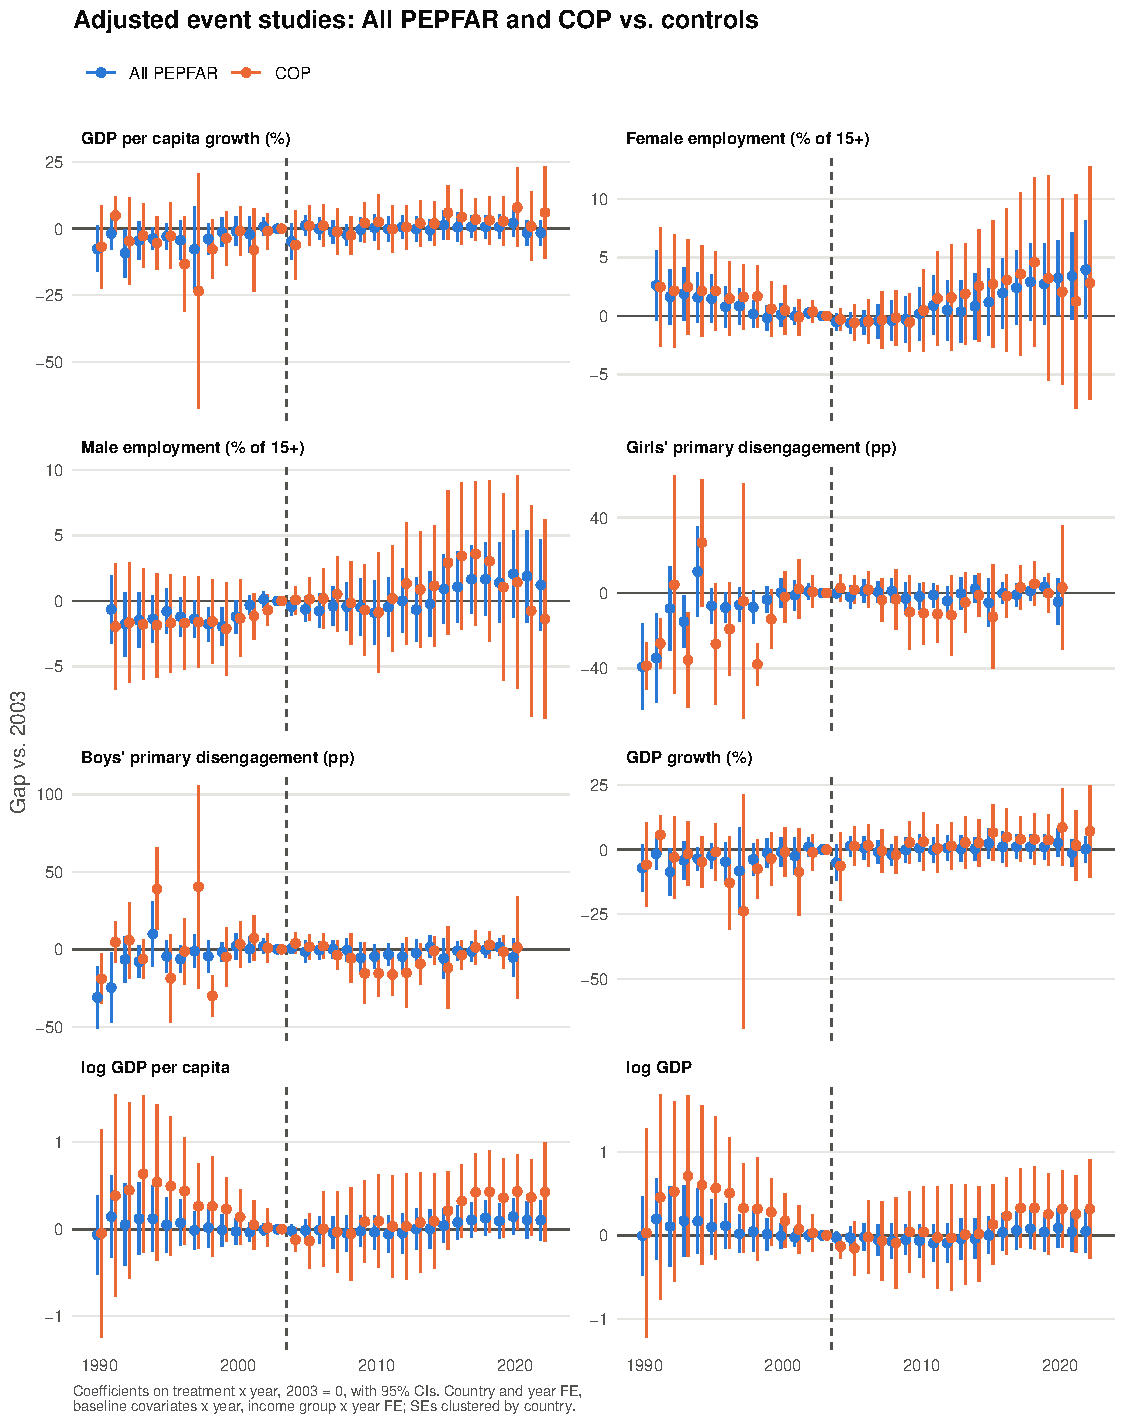
\includegraphics[width=\textwidth]{crown_event_studies/adjusted/figures/es_adj_grid_combined.pdf}
\caption{Adjusted event studies, all outcomes: All PEPFAR (blue) and COP (orange)}
\label{fig:crown_es_grid_combined}
\end{figure}
\clearpage
\begin{figure}[htbp]
\centering
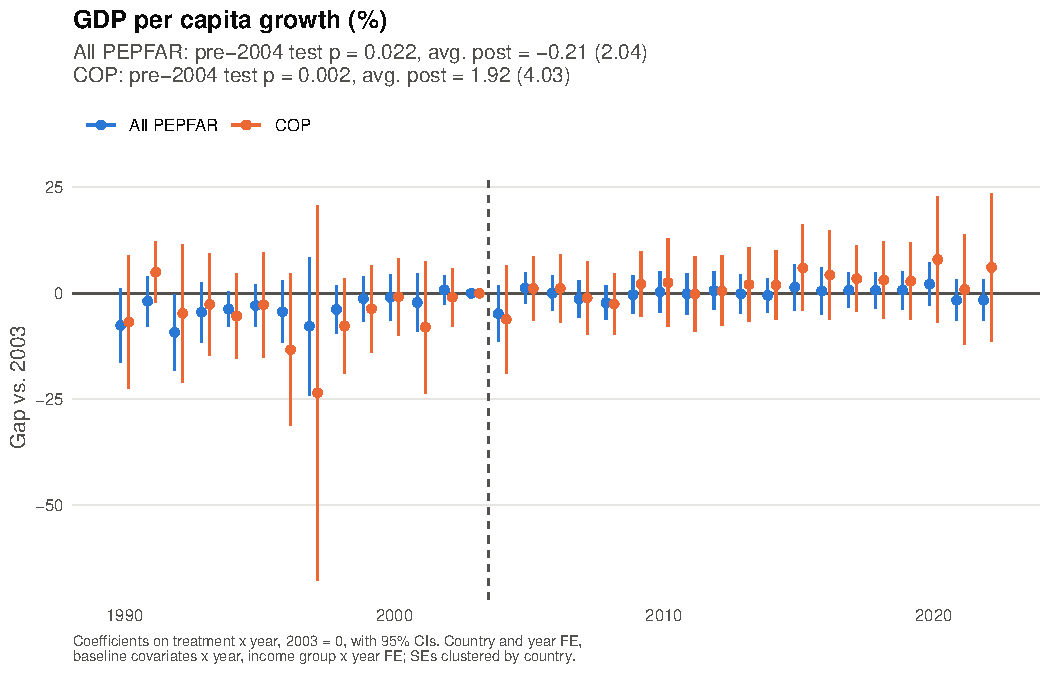
\includegraphics[width=\textwidth]{crown_event_studies/adjusted/figures/es_adj_gdp_pc_growth_combined.pdf}
\caption{Adjusted event study: GDP per capita growth (\%)}
\label{fig:crown_es_combined_gdp_pc_growth}
\end{figure}
\begin{figure}[htbp]
\centering
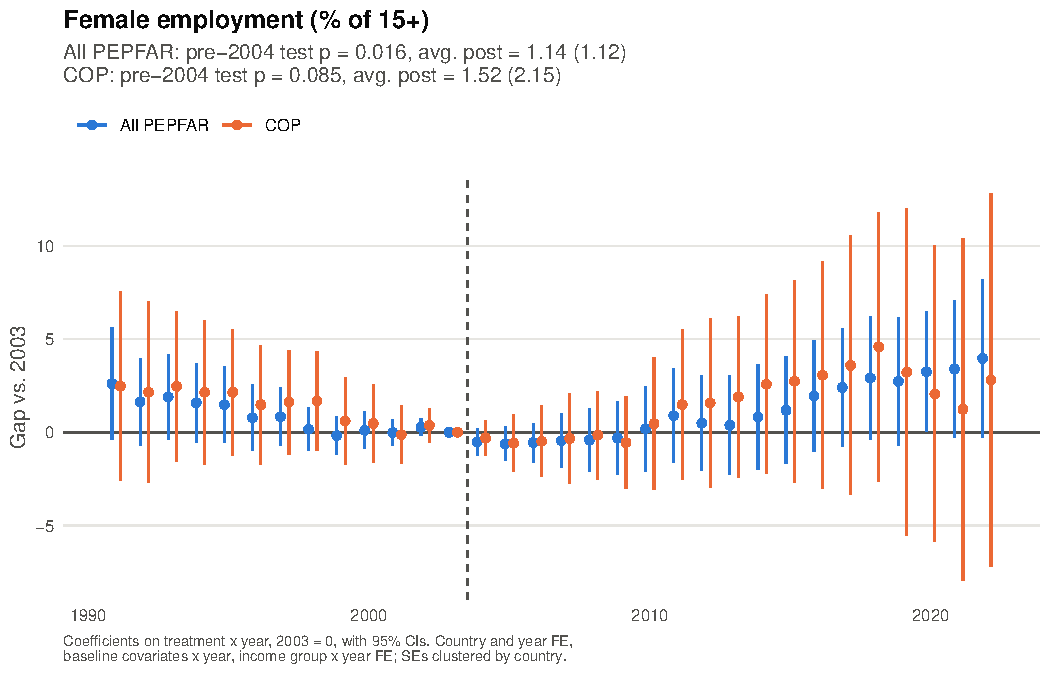
\includegraphics[width=\textwidth]{crown_event_studies/adjusted/figures/es_adj_emp_female_combined.pdf}
\caption{Adjusted event study: Female employment (\% of 15+)}
\label{fig:crown_es_combined_emp_female}
\end{figure}
\clearpage
\begin{figure}[htbp]
\centering
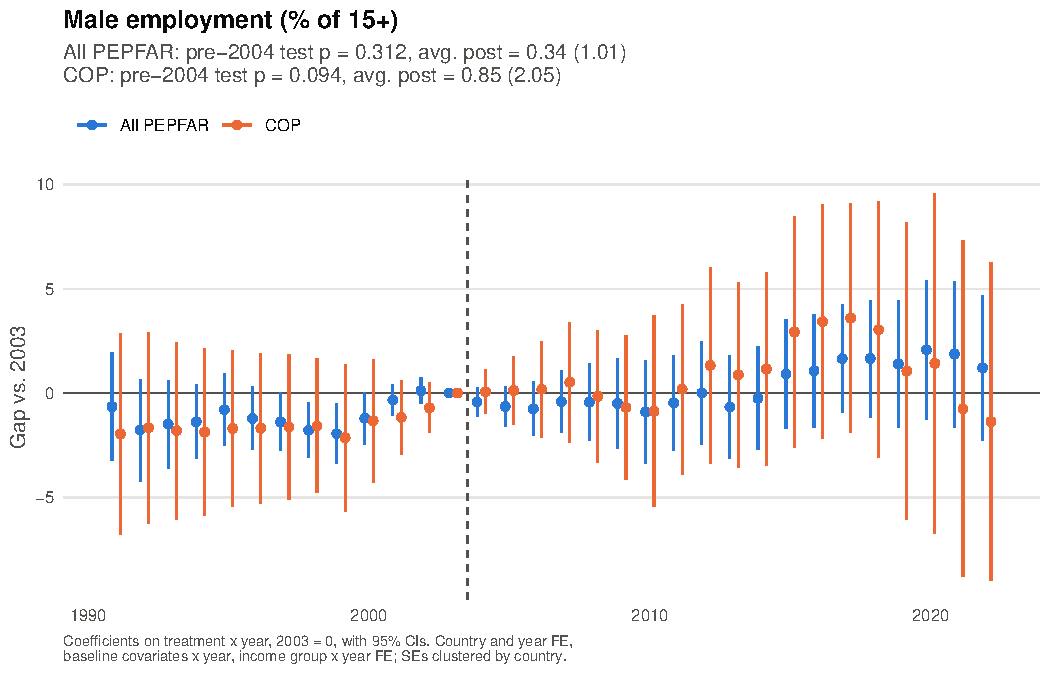
\includegraphics[width=\textwidth]{crown_event_studies/adjusted/figures/es_adj_emp_male_combined.pdf}
\caption{Adjusted event study: Male employment (\% of 15+)}
\label{fig:crown_es_combined_emp_male}
\end{figure}
\begin{figure}[htbp]
\centering
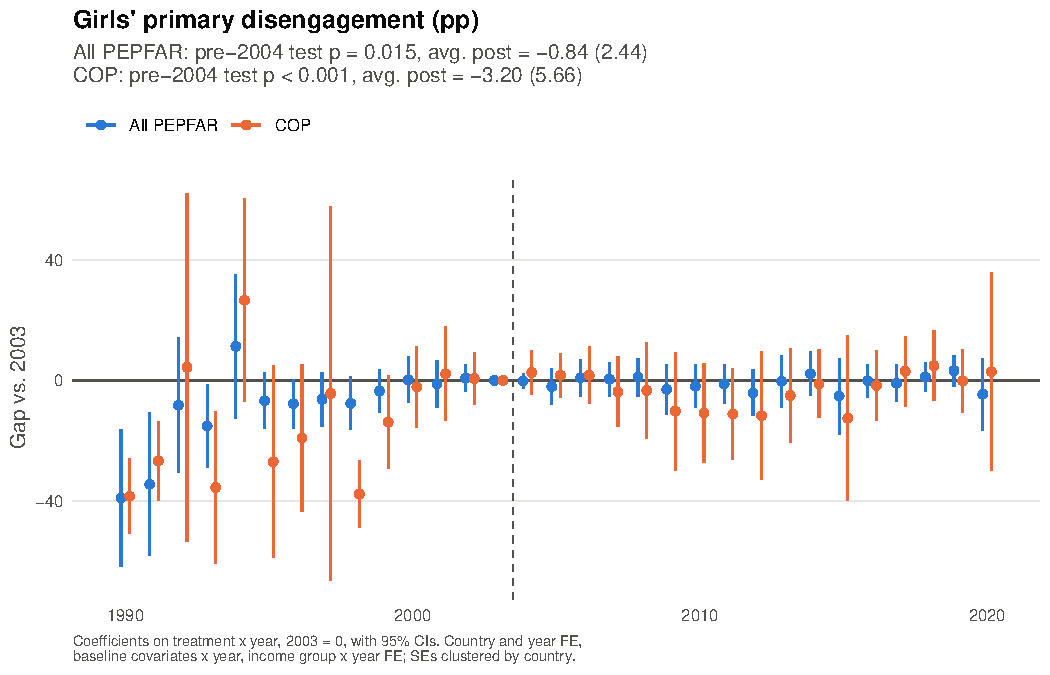
\includegraphics[width=\textwidth]{crown_event_studies/adjusted/figures/es_adj_prim_disengage_girls_combined.pdf}
\caption{Adjusted event study: Girls' primary disengagement (pp)}
\label{fig:crown_es_combined_prim_disengage_girls}
\end{figure}
\clearpage
\begin{figure}[htbp]
\centering
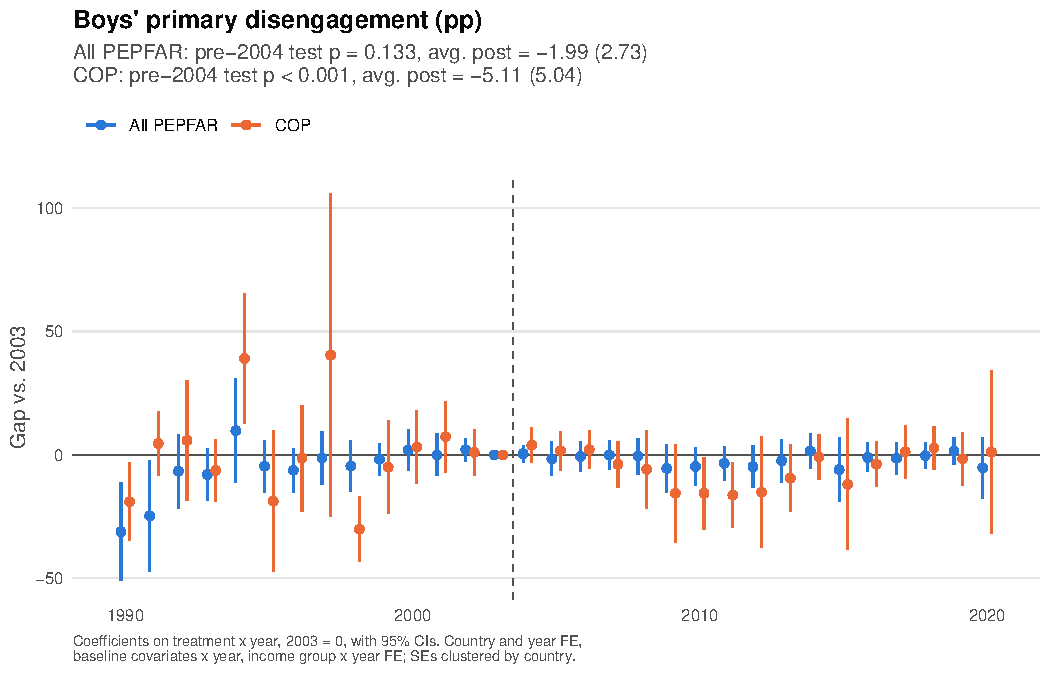
\includegraphics[width=\textwidth]{crown_event_studies/adjusted/figures/es_adj_prim_disengage_boys_combined.pdf}
\caption{Adjusted event study: Boys' primary disengagement (pp)}
\label{fig:crown_es_combined_prim_disengage_boys}
\end{figure}
\begin{figure}[htbp]
\centering
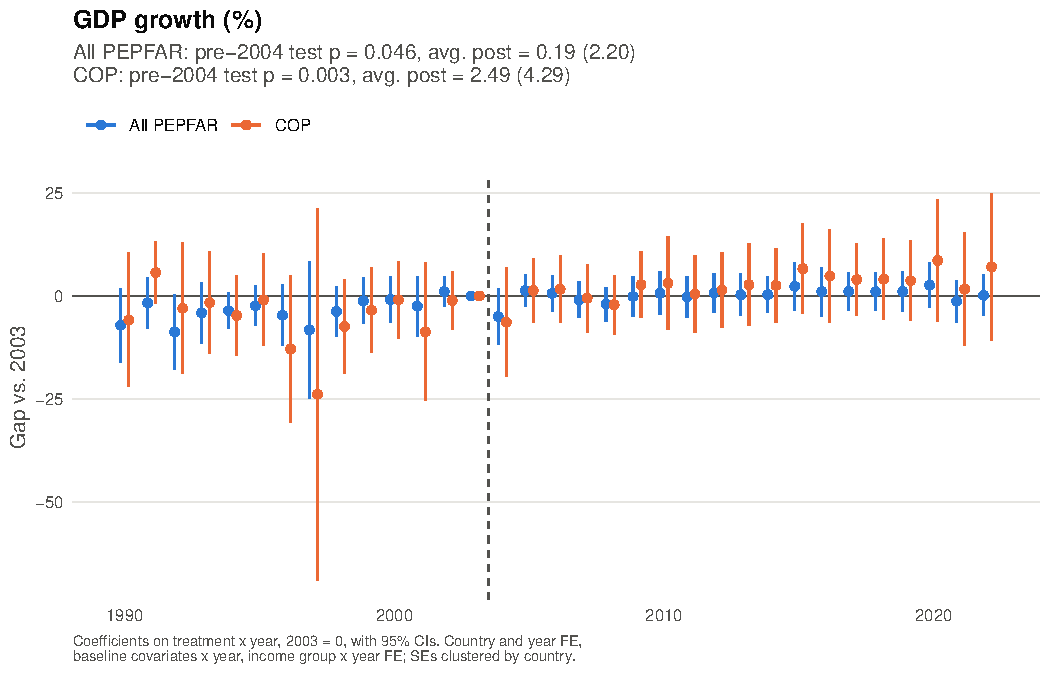
\includegraphics[width=\textwidth]{crown_event_studies/adjusted/figures/es_adj_gdp_growth_combined.pdf}
\caption{Adjusted event study: GDP growth (\%)}
\label{fig:crown_es_combined_gdp_growth}
\end{figure}
\clearpage
\begin{figure}[htbp]
\centering
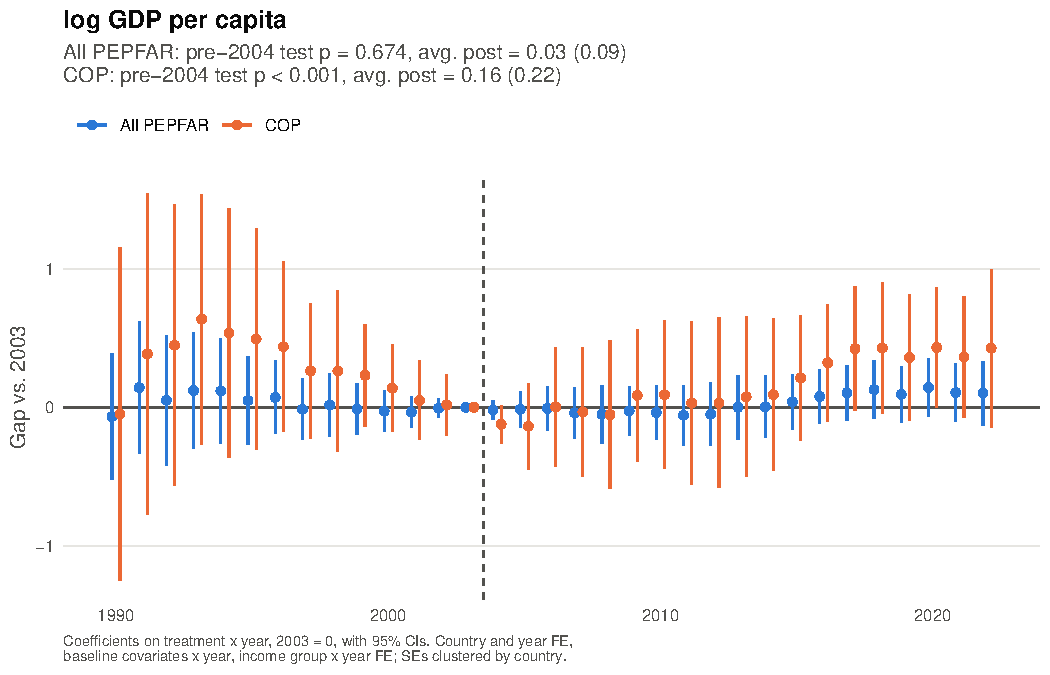
\includegraphics[width=\textwidth]{crown_event_studies/adjusted/figures/es_adj_log_gdp_pc_combined.pdf}
\caption{Adjusted event study: log GDP per capita}
\label{fig:crown_es_combined_log_gdp_pc}
\end{figure}
\begin{figure}[htbp]
\centering
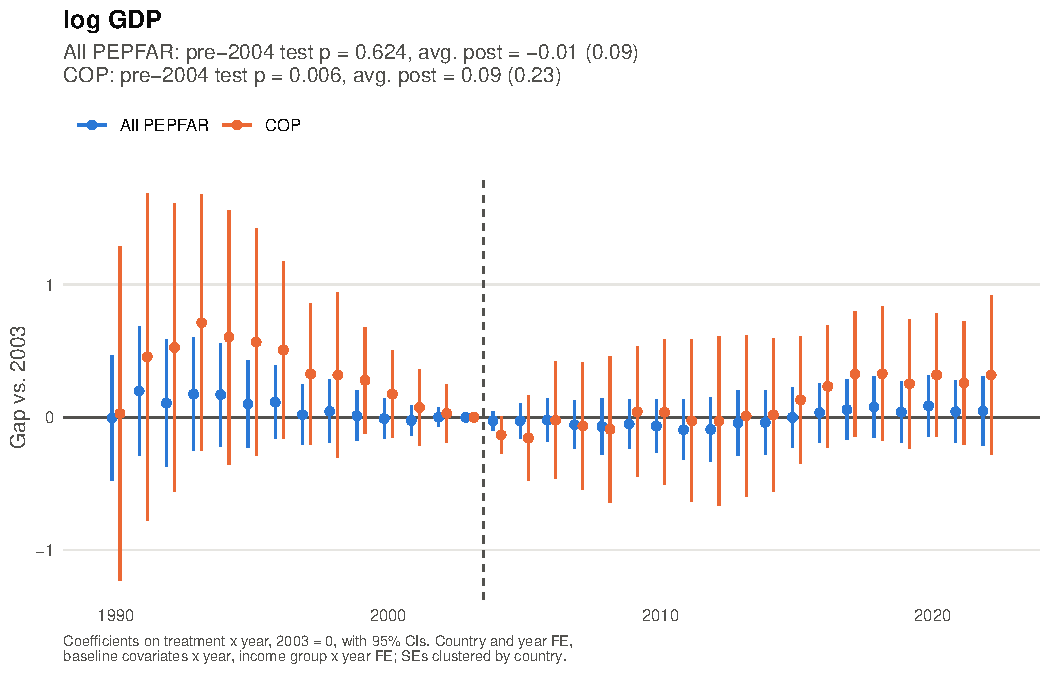
\includegraphics[width=\textwidth]{crown_event_studies/adjusted/figures/es_adj_log_gdp_combined.pdf}
\caption{Adjusted event study: log GDP}
\label{fig:crown_es_combined_log_gdp}
\end{figure}
\clearpage


\subsection{Graphs: All PEPFAR}
\begin{figure}[htbp]
\centering
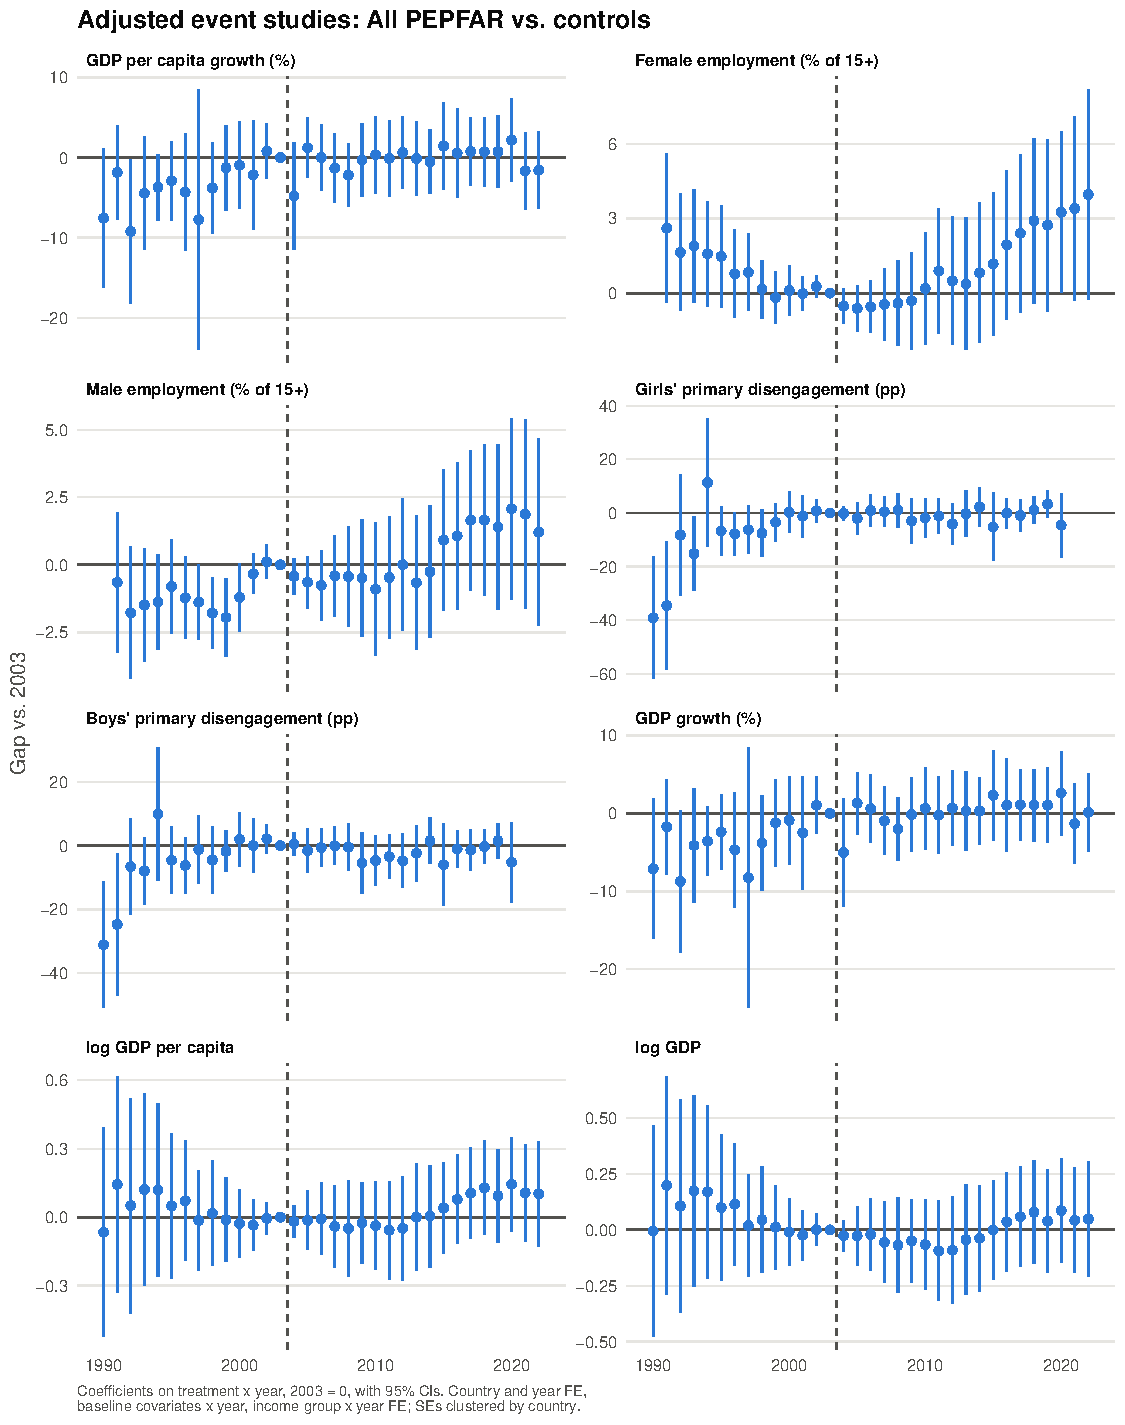
\includegraphics[width=\textwidth]{crown_event_studies/adjusted/figures/es_adj_grid_all_pepfar.pdf}
\caption{Adjusted event studies, all outcomes: All PEPFAR vs.\ controls}
\label{fig:crown_es_grid_all_pepfar}
\end{figure}
\clearpage
\begin{figure}[htbp]
\centering
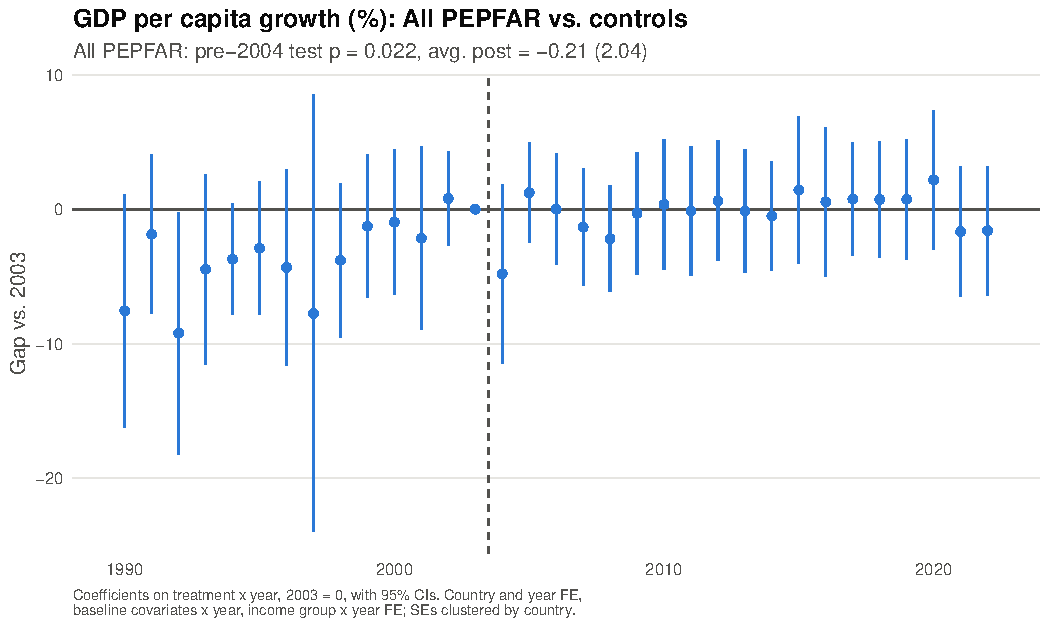
\includegraphics[width=\textwidth]{crown_event_studies/adjusted/figures/es_adj_gdp_pc_growth_all_pepfar.pdf}
\caption{Adjusted event study: GDP per capita growth (\%), All PEPFAR}
\label{fig:crown_es_all_pepfar_gdp_pc_growth}
\end{figure}
\begin{figure}[htbp]
\centering
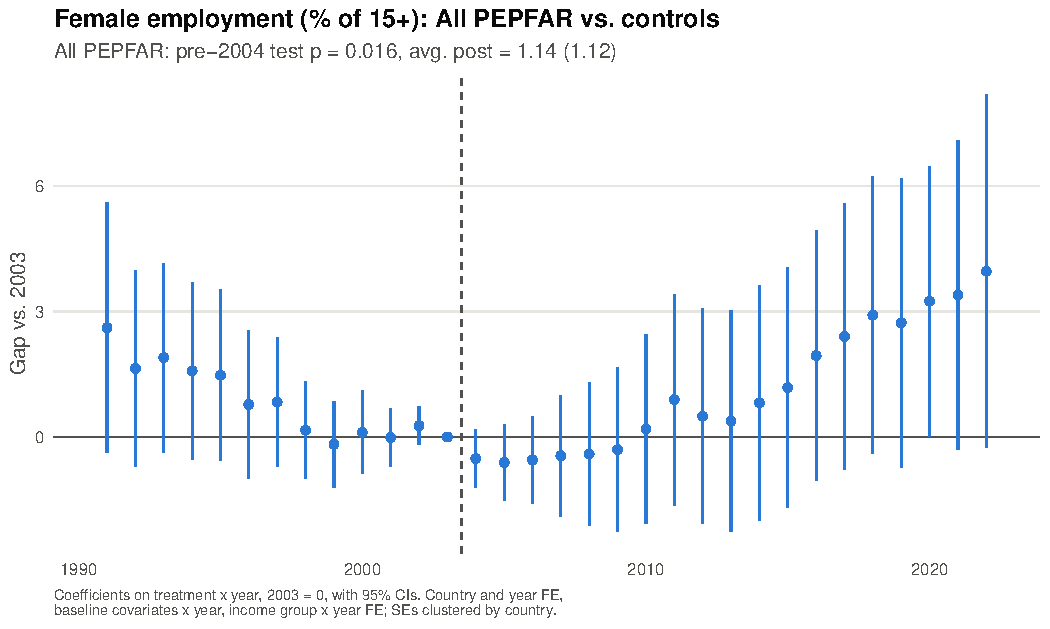
\includegraphics[width=\textwidth]{crown_event_studies/adjusted/figures/es_adj_emp_female_all_pepfar.pdf}
\caption{Adjusted event study: Female employment (\% of 15+), All PEPFAR}
\label{fig:crown_es_all_pepfar_emp_female}
\end{figure}
\clearpage
\begin{figure}[htbp]
\centering
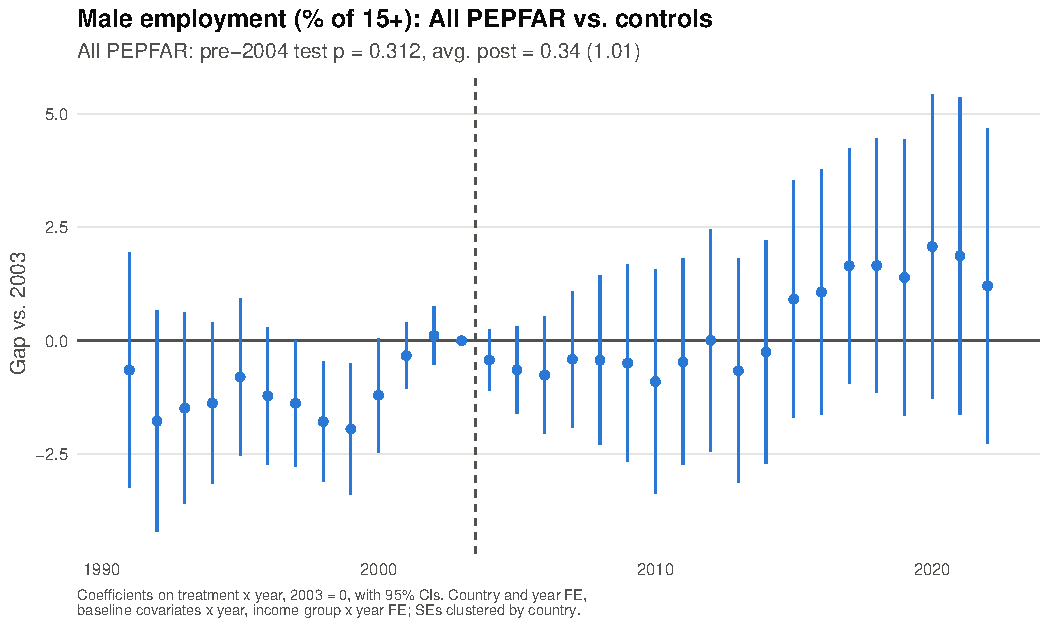
\includegraphics[width=\textwidth]{crown_event_studies/adjusted/figures/es_adj_emp_male_all_pepfar.pdf}
\caption{Adjusted event study: Male employment (\% of 15+), All PEPFAR}
\label{fig:crown_es_all_pepfar_emp_male}
\end{figure}
\begin{figure}[htbp]
\centering
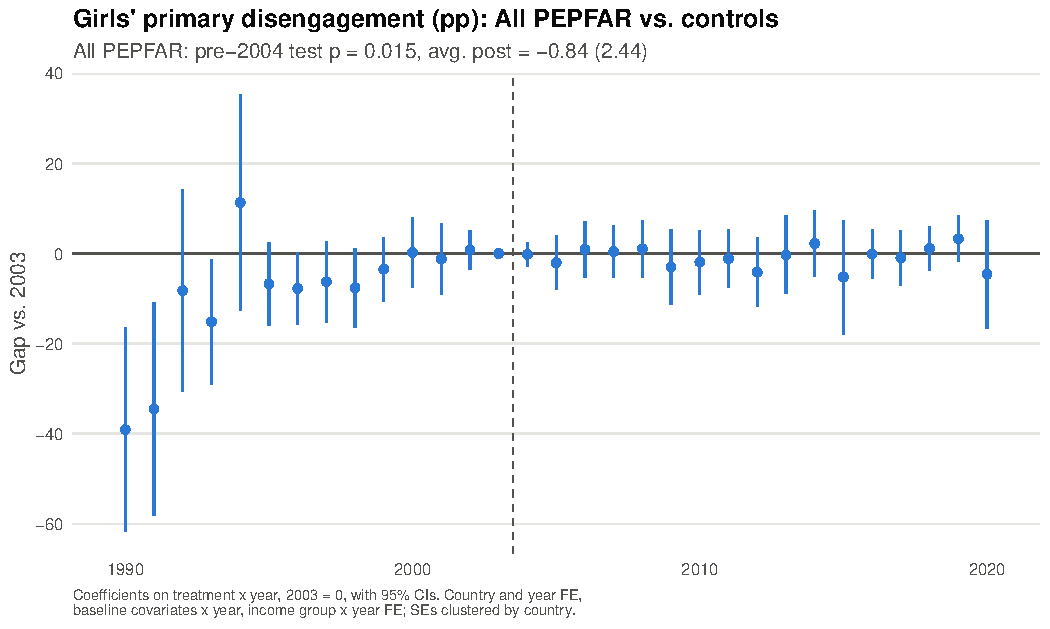
\includegraphics[width=\textwidth]{crown_event_studies/adjusted/figures/es_adj_prim_disengage_girls_all_pepfar.pdf}
\caption{Adjusted event study: Girls' primary disengagement (pp), All PEPFAR}
\label{fig:crown_es_all_pepfar_prim_disengage_girls}
\end{figure}
\clearpage
\begin{figure}[htbp]
\centering
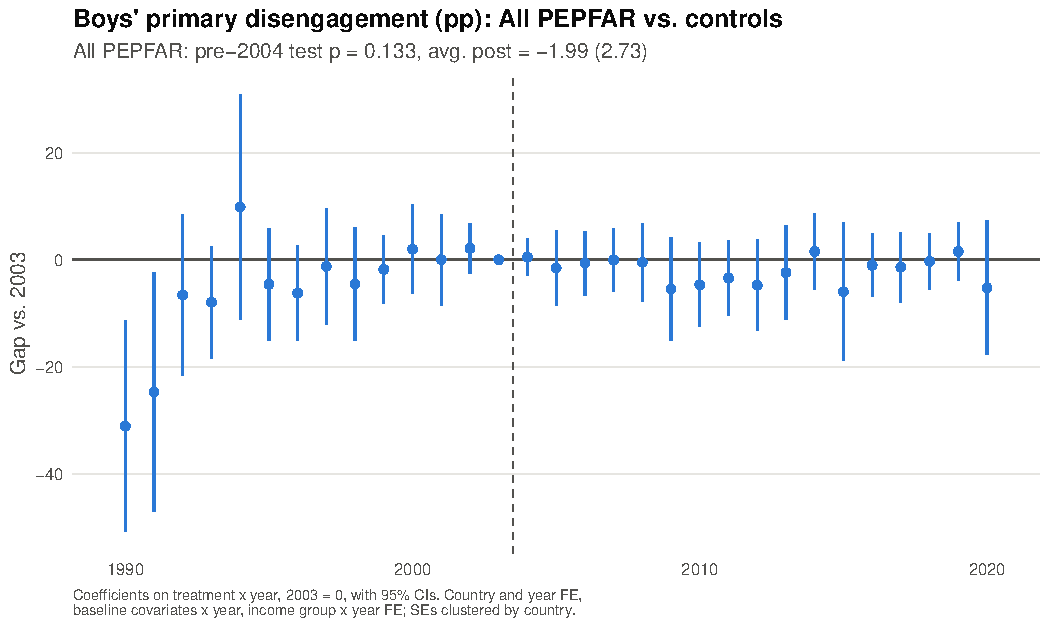
\includegraphics[width=\textwidth]{crown_event_studies/adjusted/figures/es_adj_prim_disengage_boys_all_pepfar.pdf}
\caption{Adjusted event study: Boys' primary disengagement (pp), All PEPFAR}
\label{fig:crown_es_all_pepfar_prim_disengage_boys}
\end{figure}
\begin{figure}[htbp]
\centering
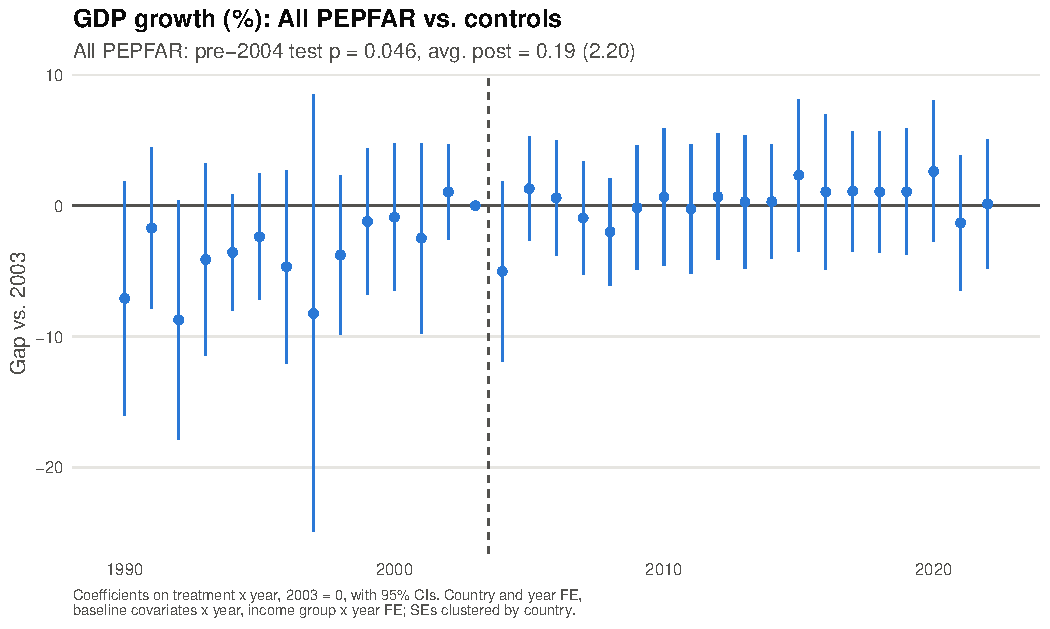
\includegraphics[width=\textwidth]{crown_event_studies/adjusted/figures/es_adj_gdp_growth_all_pepfar.pdf}
\caption{Adjusted event study: GDP growth (\%), All PEPFAR}
\label{fig:crown_es_all_pepfar_gdp_growth}
\end{figure}
\clearpage
\begin{figure}[htbp]
\centering
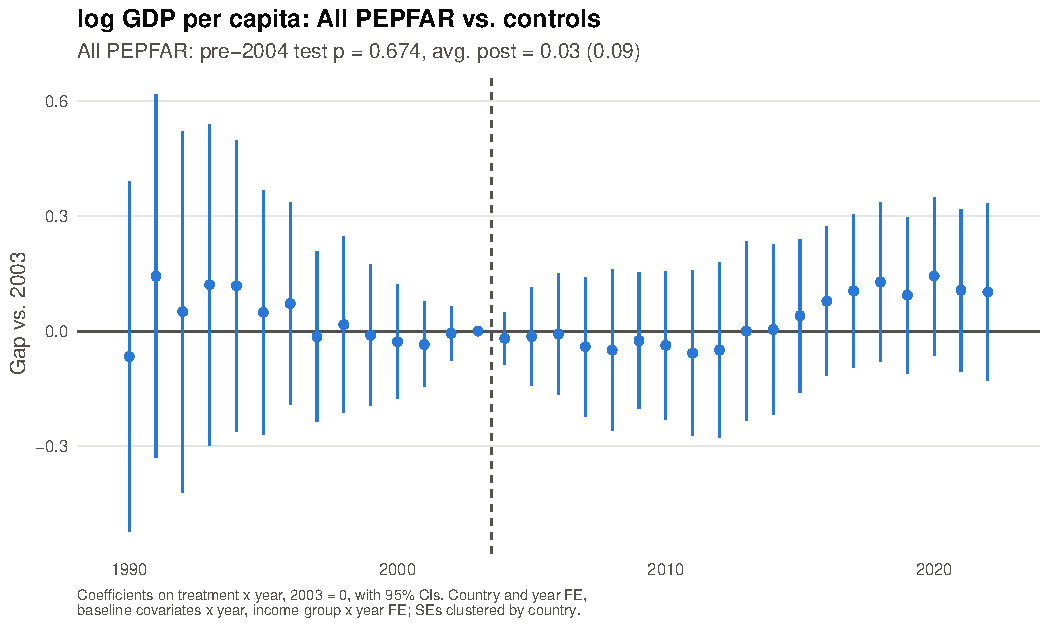
\includegraphics[width=\textwidth]{crown_event_studies/adjusted/figures/es_adj_log_gdp_pc_all_pepfar.pdf}
\caption{Adjusted event study: log GDP per capita, All PEPFAR}
\label{fig:crown_es_all_pepfar_log_gdp_pc}
\end{figure}
\begin{figure}[htbp]
\centering
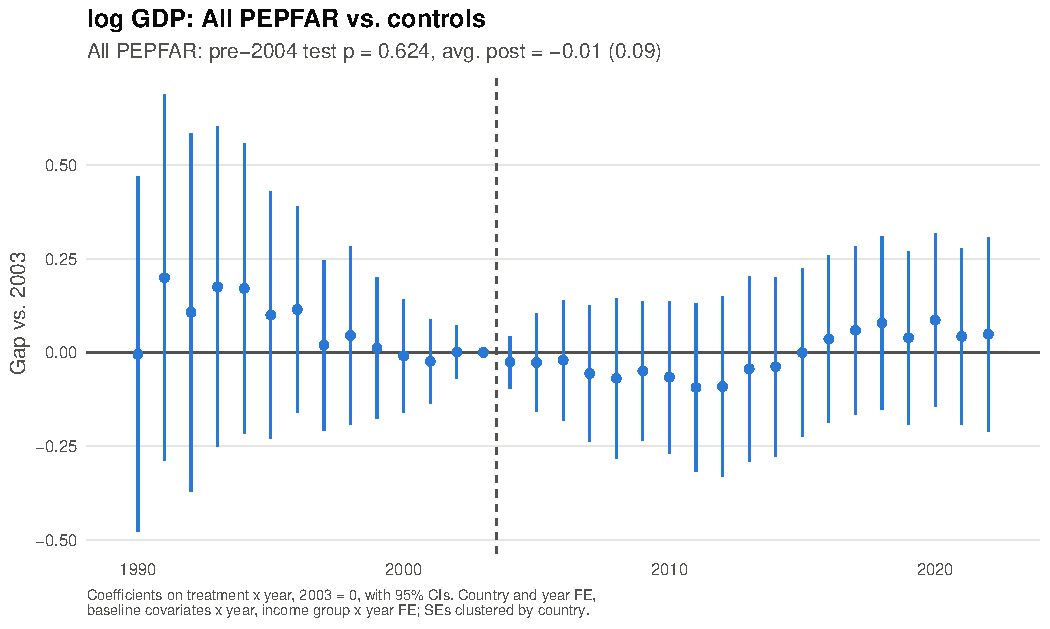
\includegraphics[width=\textwidth]{crown_event_studies/adjusted/figures/es_adj_log_gdp_all_pepfar.pdf}
\caption{Adjusted event study: log GDP, All PEPFAR}
\label{fig:crown_es_all_pepfar_log_gdp}
\end{figure}
\clearpage


\subsection{Graphs: COP}
\begin{figure}[htbp]
\centering
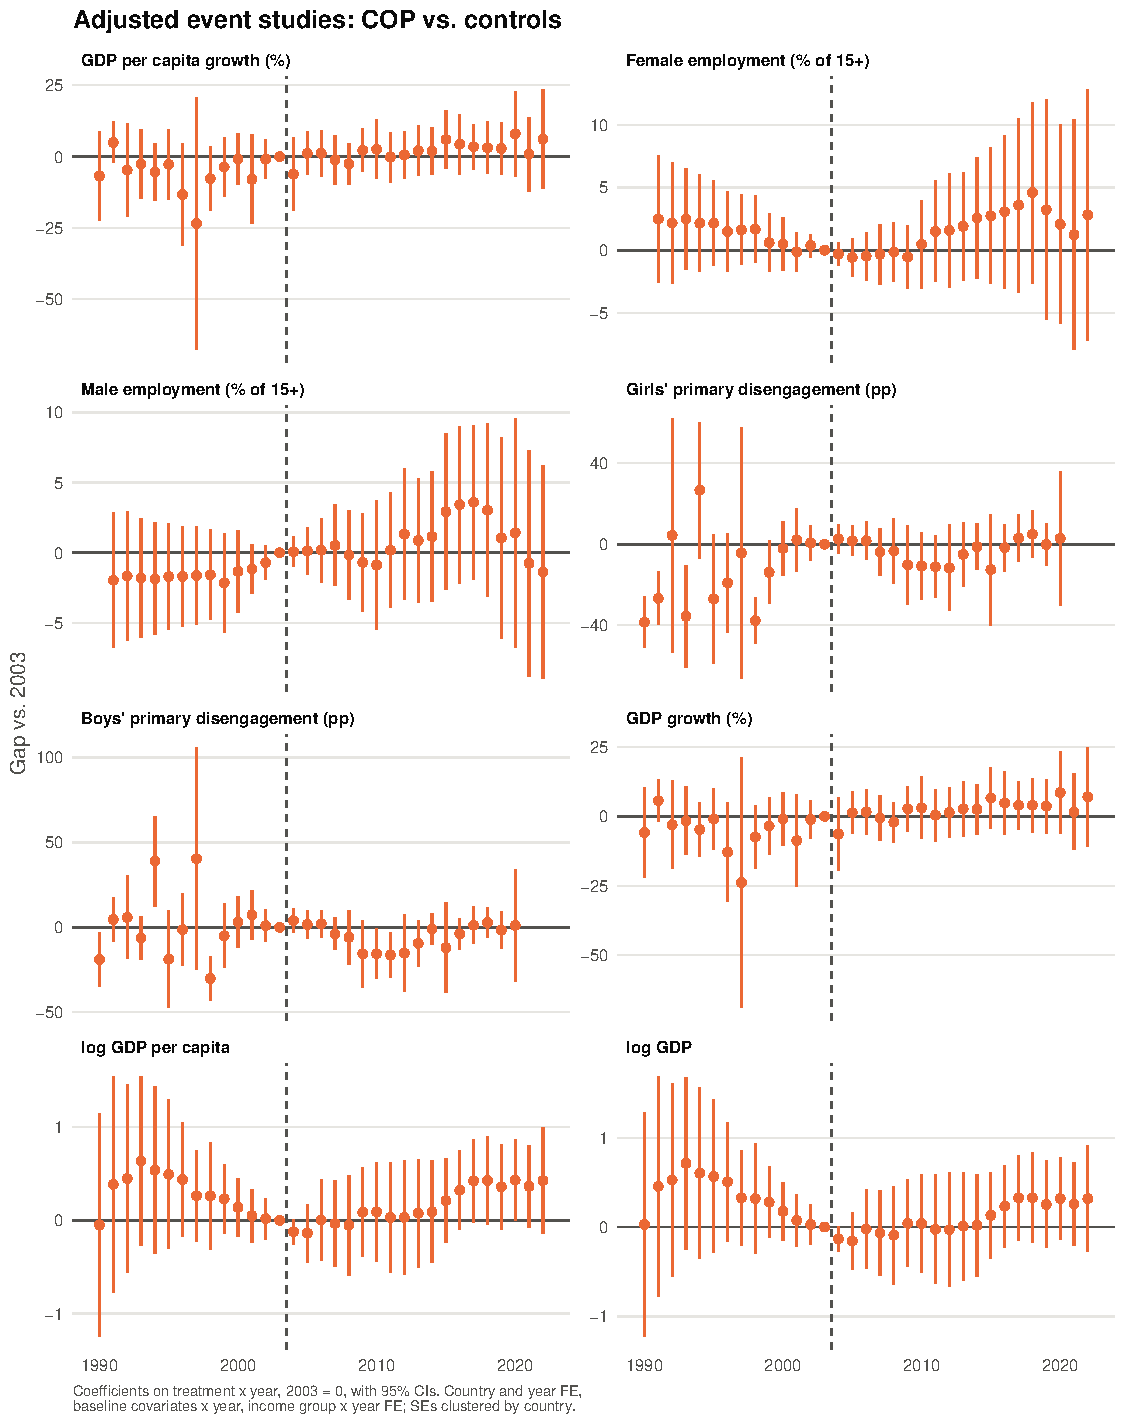
\includegraphics[width=\textwidth]{crown_event_studies/adjusted/figures/es_adj_grid_cop.pdf}
\caption{Adjusted event studies, all outcomes: COP vs.\ controls}
\label{fig:crown_es_grid_cop}
\end{figure}
\clearpage
\begin{figure}[htbp]
\centering
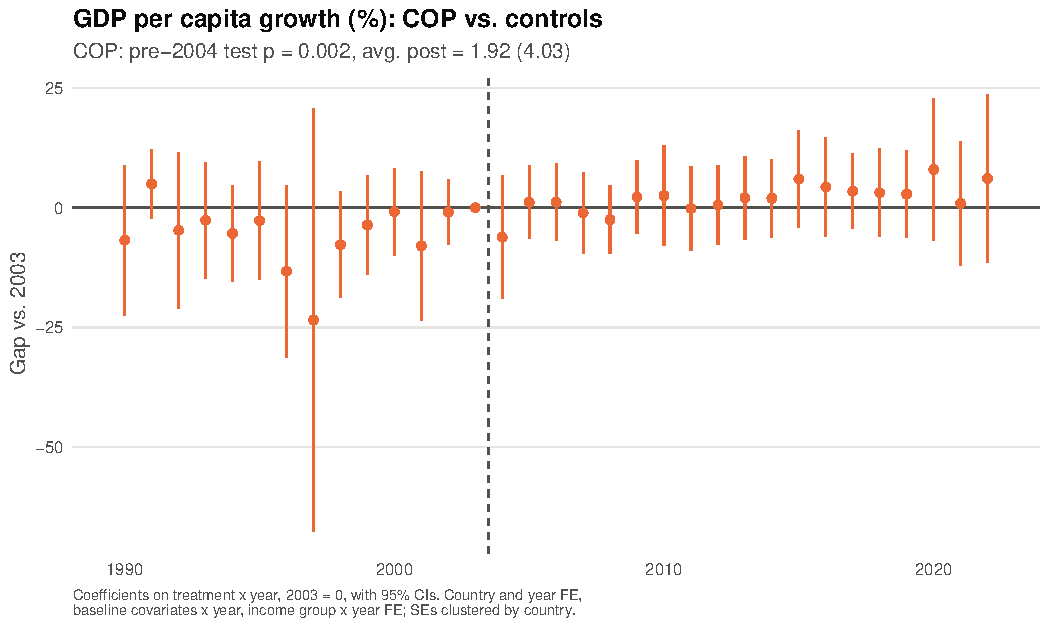
\includegraphics[width=\textwidth]{crown_event_studies/adjusted/figures/es_adj_gdp_pc_growth_cop.pdf}
\caption{Adjusted event study: GDP per capita growth (\%), COP}
\label{fig:crown_es_cop_gdp_pc_growth}
\end{figure}
\begin{figure}[htbp]
\centering
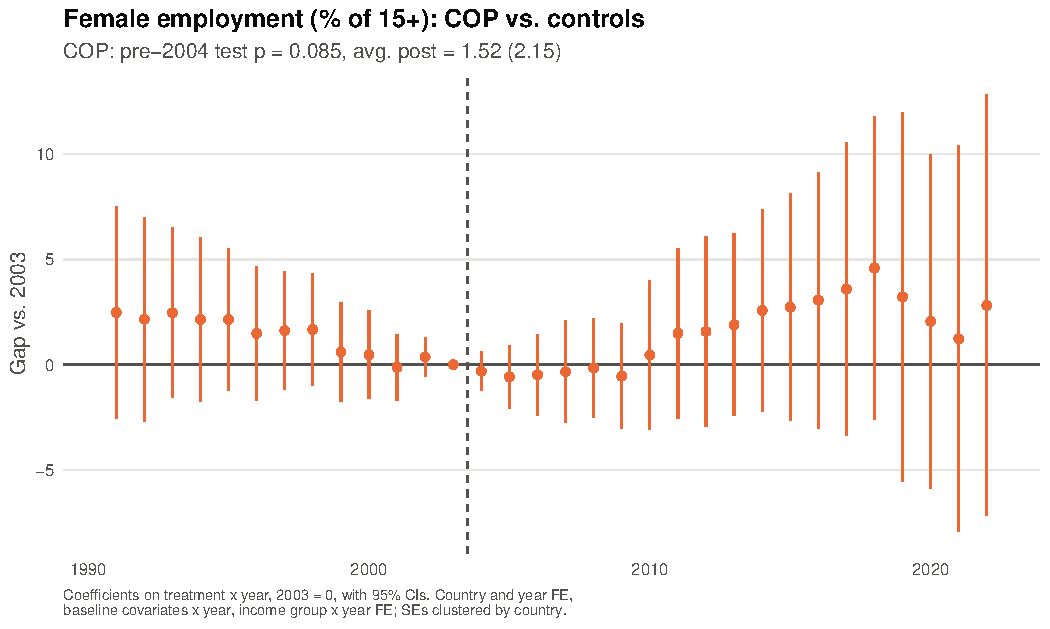
\includegraphics[width=\textwidth]{crown_event_studies/adjusted/figures/es_adj_emp_female_cop.pdf}
\caption{Adjusted event study: Female employment (\% of 15+), COP}
\label{fig:crown_es_cop_emp_female}
\end{figure}
\clearpage
\begin{figure}[htbp]
\centering
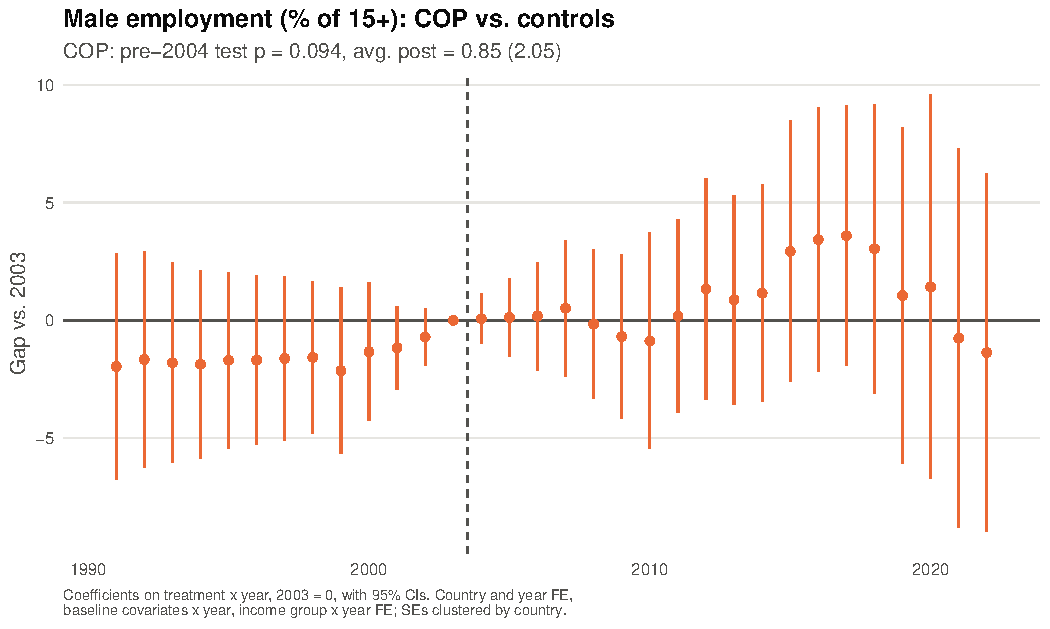
\includegraphics[width=\textwidth]{crown_event_studies/adjusted/figures/es_adj_emp_male_cop.pdf}
\caption{Adjusted event study: Male employment (\% of 15+), COP}
\label{fig:crown_es_cop_emp_male}
\end{figure}
\begin{figure}[htbp]
\centering
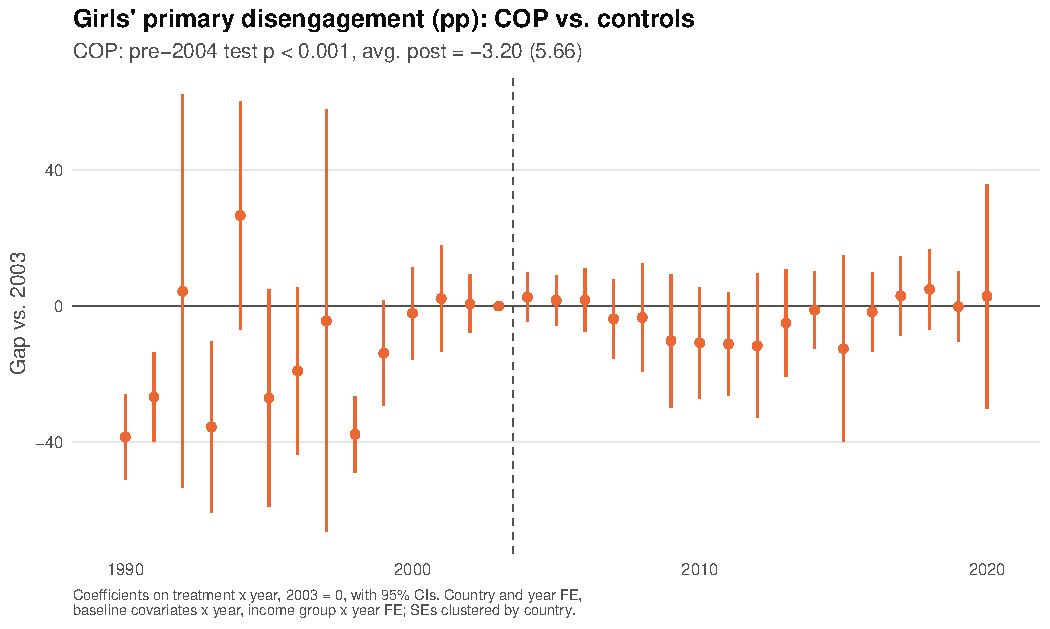
\includegraphics[width=\textwidth]{crown_event_studies/adjusted/figures/es_adj_prim_disengage_girls_cop.pdf}
\caption{Adjusted event study: Girls' primary disengagement (pp), COP}
\label{fig:crown_es_cop_prim_disengage_girls}
\end{figure}
\clearpage
\begin{figure}[htbp]
\centering
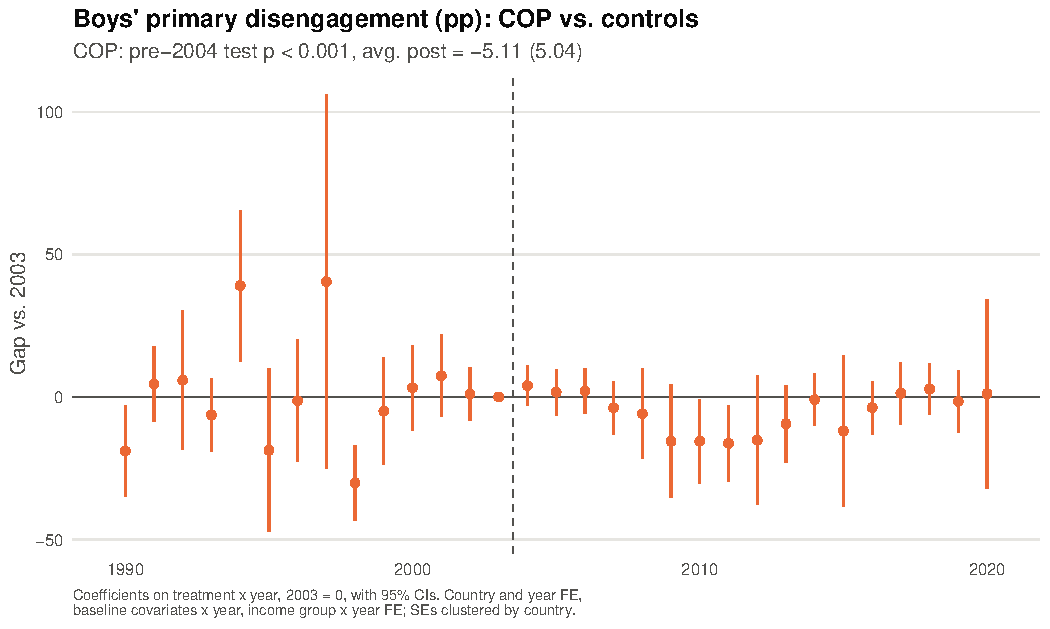
\includegraphics[width=\textwidth]{crown_event_studies/adjusted/figures/es_adj_prim_disengage_boys_cop.pdf}
\caption{Adjusted event study: Boys' primary disengagement (pp), COP}
\label{fig:crown_es_cop_prim_disengage_boys}
\end{figure}
\begin{figure}[htbp]
\centering
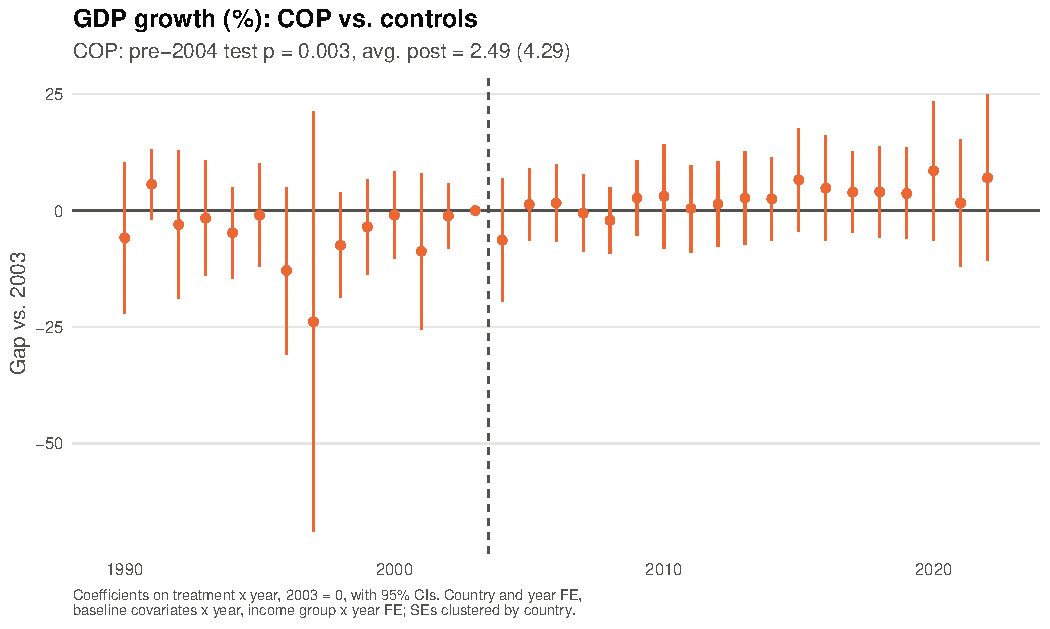
\includegraphics[width=\textwidth]{crown_event_studies/adjusted/figures/es_adj_gdp_growth_cop.pdf}
\caption{Adjusted event study: GDP growth (\%), COP}
\label{fig:crown_es_cop_gdp_growth}
\end{figure}
\clearpage
\begin{figure}[htbp]
\centering
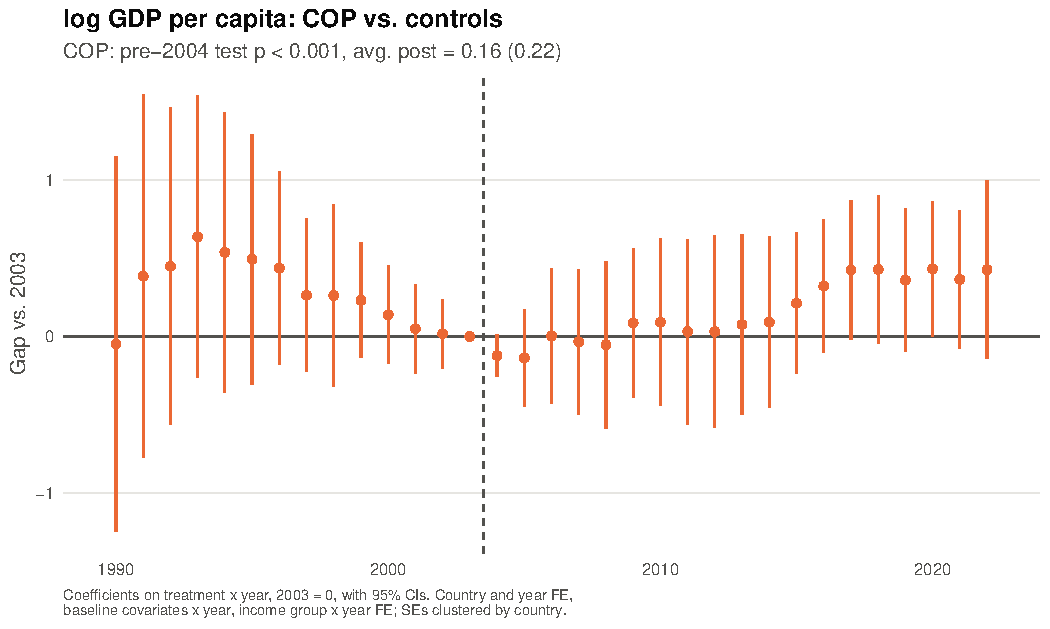
\includegraphics[width=\textwidth]{crown_event_studies/adjusted/figures/es_adj_log_gdp_pc_cop.pdf}
\caption{Adjusted event study: log GDP per capita, COP}
\label{fig:crown_es_cop_log_gdp_pc}
\end{figure}
\begin{figure}[htbp]
\centering
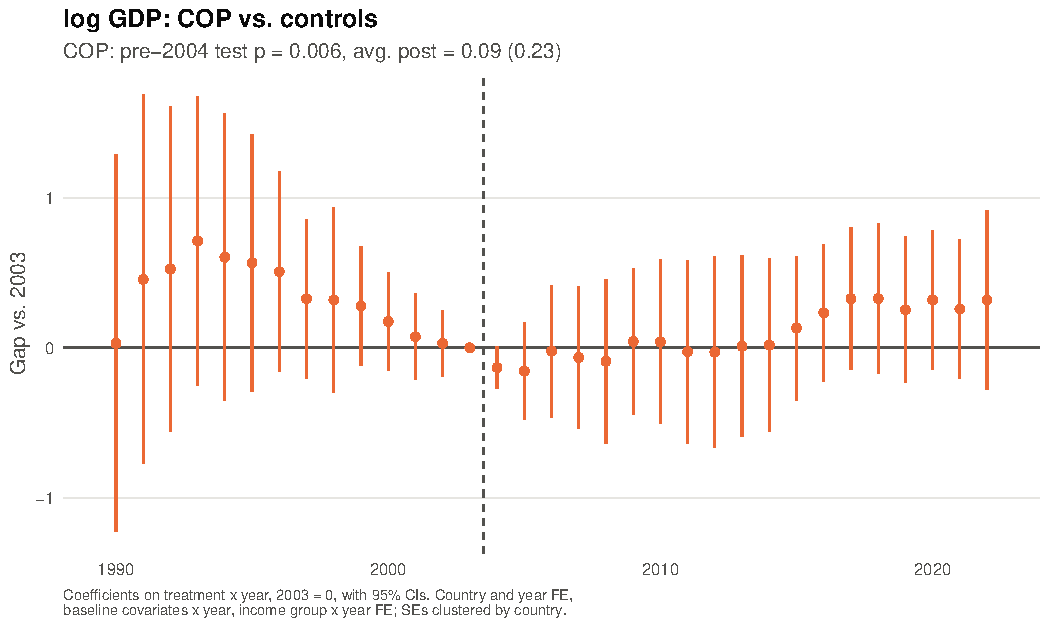
\includegraphics[width=\textwidth]{crown_event_studies/adjusted/figures/es_adj_log_gdp_cop.pdf}
\caption{Adjusted event study: log GDP, COP}
\label{fig:crown_es_cop_log_gdp}
\end{figure}
\clearpage


\subsection{Tables: All PEPFAR and COP together}
\begin{table}[htbp]
\centering
\small
\caption{Adjusted event study: GDP pc growth, All PEPFAR and COP}
\label{tab:crown_es_combined_gdp_pc_growth}
\begin{tabular}{lcccc}
\toprule
 & \multicolumn{2}{c}{All PEPFAR vs.\ controls} & \multicolumn{2}{c}{COP vs.\ controls} \\
\cmidrule(lr){2-3}\cmidrule(lr){4-5}
Year & Coef. & SE & Coef. & SE \\
\midrule
1990 & $-7.563^{*}$ & (4.426) & $-6.780$ & (7.995) \\
1991 & $-1.863$ & (3.008) & $4.958$ & (3.670) \\
1992 & $-9.219^{**}$ & (4.590) & $-4.725$ & (8.326) \\
1993 & $-4.462$ & (3.609) & $-2.619$ & (6.180) \\
1994 & $-3.719^{*}$ & (2.110) & $-5.387$ & (5.092) \\
1995 & $-2.903$ & (2.531) & $-2.703$ & (6.315) \\
1996 & $-4.328$ & (3.734) & $-13.291$ & (9.160) \\
1997 & $-7.753$ & (8.290) & $-23.467$ & (22.585) \\
1998 & $-3.802$ & (2.928) & $-7.732$ & (5.671) \\
1999 & $-1.270$ & (2.718) & $-3.624$ & (5.245) \\
2000 & $-0.965$ & (2.762) & $-0.819$ & (4.633) \\
2001 & $-2.165$ & (3.474) & $-7.967$ & (7.948) \\
2002 & $0.797$ & (1.770) & $-0.927$ & (3.485) \\
2003 & \multicolumn{2}{c}{(reference)} & \multicolumn{2}{c}{(reference)} \\
2004 & $-4.799$ & (3.392) & $-6.133$ & (6.536) \\
2005 & $1.229$ & (1.909) & $1.138$ & (3.866) \\
2006 & $0.002$ & (2.102) & $1.155$ & (4.094) \\
2007 & $-1.334$ & (2.211) & $-1.101$ & (4.363) \\
2008 & $-2.193$ & (2.018) & $-2.507$ & (3.629) \\
2009 & $-0.303$ & (2.312) & $2.209$ & (3.869) \\
2010 & $0.354$ & (2.452) & $2.533$ & (5.291) \\
2011 & $-0.118$ & (2.449) & $-0.166$ & (4.487) \\
2012 & $0.625$ & (2.277) & $0.590$ & (4.212) \\
2013 & $-0.127$ & (2.339) & $2.080$ & (4.447) \\
2014 & $-0.509$ & (2.057) & $1.958$ & (4.170) \\
2015 & $1.434$ & (2.784) & $5.998$ & (5.176) \\
2016 & $0.550$ & (2.823) & $4.325$ & (5.327) \\
2017 & $0.755$ & (2.140) & $3.452$ & (3.989) \\
2018 & $0.723$ & (2.194) & $3.136$ & (4.661) \\
2019 & $0.737$ & (2.282) & $2.844$ & (4.648) \\
2020 & $2.174$ & (2.635) & $7.979$ & (7.577) \\
2021 & $-1.660$ & (2.465) & $0.890$ & (6.607) \\
2022 & $-1.591$ & (2.445) & $6.098$ & (8.901) \\
\midrule
Pre-2004 joint test ($p$) & \multicolumn{2}{c}{0.022} & \multicolumn{2}{c}{0.002} \\
Average 2004--2022 & $-0.213$ & (2.038) & $1.920$ & (4.030) \\
Observations & \multicolumn{2}{c}{3,392} & \multicolumn{2}{c}{1,903} \\
Countries & \multicolumn{2}{c}{104} & \multicolumn{2}{c}{58} \\
\bottomrule
\end{tabular}
\par\vspace{4pt}
\begin{minipage}{\textwidth}\footnotesize Coefficients on treatment group $\times$ year, relative to 2003 (omitted); standard errors clustered by country in parentheses. All models include country and year fixed effects, the 11 baseline (2003) covariates of Crown et al.\ (2023) each with its own coefficient in every year, and World Bank income group $\times$ year fixed effects. Sample 1990--2022; controls are the 64 comparison countries valid through 2022 (\texttt{grp\_control\_kates}). Blank cells: no data for that outcome in that year. Disengagement is in percentage points. $^{*}p<0.10$, $^{**}p<0.05$, $^{***}p<0.01$.\end{minipage}
\end{table}

\clearpage
\begin{table}[htbp]
\centering
\small
\caption{Adjusted event study: Female emp., All PEPFAR and COP}
\label{tab:crown_es_combined_emp_female}
\begin{tabular}{lcccc}
\toprule
 & \multicolumn{2}{c}{All PEPFAR vs.\ controls} & \multicolumn{2}{c}{COP vs.\ controls} \\
\cmidrule(lr){2-3}\cmidrule(lr){4-5}
Year & Coef. & SE & Coef. & SE \\
\midrule
1991 & $2.614^{*}$ & (1.525) & $2.480$ & (2.580) \\
1992 & $1.638$ & (1.197) & $2.155$ & (2.470) \\
1993 & $1.899$ & (1.154) & $2.466$ & (2.056) \\
1994 & $1.584$ & (1.081) & $2.146$ & (1.976) \\
1995 & $1.478$ & (1.046) & $2.146$ & (1.721) \\
1996 & $0.776$ & (0.902) & $1.484$ & (1.625) \\
1997 & $0.835$ & (0.789) & $1.618$ & (1.426) \\
1998 & $0.162$ & (0.593) & $1.672$ & (1.354) \\
1999 & $-0.177$ & (0.526) & $0.604$ & (1.189) \\
2000 & $0.108$ & (0.507) & $0.473$ & (1.069) \\
2001 & $-0.015$ & (0.353) & $-0.128$ & (0.794) \\
2002 & $0.269$ & (0.232) & $0.368$ & (0.467) \\
2003 & \multicolumn{2}{c}{(reference)} & \multicolumn{2}{c}{(reference)} \\
2004 & $-0.518$ & (0.359) & $-0.308$ & (0.476) \\
2005 & $-0.611$ & (0.464) & $-0.582$ & (0.773) \\
2006 & $-0.549$ & (0.533) & $-0.482$ & (0.975) \\
2007 & $-0.449$ & (0.741) & $-0.333$ & (1.233) \\
2008 & $-0.408$ & (0.874) & $-0.157$ & (1.203) \\
2009 & $-0.302$ & (0.998) & $-0.548$ & (1.268) \\
2010 & $0.188$ & (1.157) & $0.462$ & (1.801) \\
2011 & $0.893$ & (1.286) & $1.491$ & (2.057) \\
2012 & $0.495$ & (1.309) & $1.575$ & (2.308) \\
2013 & $0.377$ & (1.352) & $1.897$ & (2.211) \\
2014 & $0.818$ & (1.435) & $2.574$ & (2.450) \\
2015 & $1.180$ & (1.469) & $2.737$ & (2.761) \\
2016 & $1.946$ & (1.528) & $3.066$ & (3.106) \\
2017 & $2.405$ & (1.624) & $3.589$ & (3.543) \\
2018 & $2.912^{*}$ & (1.688) & $4.588$ & (3.680) \\
2019 & $2.733$ & (1.761) & $3.221$ & (4.476) \\
2020 & $3.248^{*}$ & (1.648) & $2.058$ & (4.051) \\
2021 & $3.400^{*}$ & (1.887) & $1.231$ & (4.683) \\
2022 & $3.963^{*}$ & (2.152) & $2.814$ & (5.101) \\
\midrule
Pre-2004 joint test ($p$) & \multicolumn{2}{c}{0.016} & \multicolumn{2}{c}{0.085} \\
Average 2004--2022 & $1.143$ & (1.122) & $1.521$ & (2.152) \\
Observations & \multicolumn{2}{c}{3,136} & \multicolumn{2}{c}{1,696} \\
Countries & \multicolumn{2}{c}{98} & \multicolumn{2}{c}{53} \\
\bottomrule
\end{tabular}
\par\vspace{4pt}
\begin{minipage}{\textwidth}\footnotesize Coefficients on treatment group $\times$ year, relative to 2003 (omitted); standard errors clustered by country in parentheses. All models include country and year fixed effects, the 11 baseline (2003) covariates of Crown et al.\ (2023) each with its own coefficient in every year, and World Bank income group $\times$ year fixed effects. Sample 1990--2022; controls are the 64 comparison countries valid through 2022 (\texttt{grp\_control\_kates}). Blank cells: no data for that outcome in that year. Disengagement is in percentage points. $^{*}p<0.10$, $^{**}p<0.05$, $^{***}p<0.01$.\end{minipage}
\end{table}

\clearpage
\begin{table}[htbp]
\centering
\small
\caption{Adjusted event study: Male emp., All PEPFAR and COP}
\label{tab:crown_es_combined_emp_male}
\begin{tabular}{lcccc}
\toprule
 & \multicolumn{2}{c}{All PEPFAR vs.\ controls} & \multicolumn{2}{c}{COP vs.\ controls} \\
\cmidrule(lr){2-3}\cmidrule(lr){4-5}
Year & Coef. & SE & Coef. & SE \\
\midrule
1991 & $-0.648$ & (1.323) & $-1.959$ & (2.457) \\
1992 & $-1.776$ & (1.246) & $-1.661$ & (2.334) \\
1993 & $-1.487$ & (1.076) & $-1.799$ & (2.164) \\
1994 & $-1.377$ & (0.904) & $-1.868$ & (2.035) \\
1995 & $-0.801$ & (0.881) & $-1.697$ & (1.911) \\
1996 & $-1.217$ & (0.770) & $-1.687$ & (1.829) \\
1997 & $-1.382^{*}$ & (0.709) & $-1.617$ & (1.768) \\
1998 & $-1.785^{***}$ & (0.672) & $-1.569$ & (1.642) \\
1999 & $-1.948^{***}$ & (0.732) & $-2.136$ & (1.801) \\
2000 & $-1.204^{*}$ & (0.641) & $-1.332$ & (1.497) \\
2001 & $-0.331$ & (0.374) & $-1.163$ & (0.900) \\
2002 & $0.113$ & (0.324) & $-0.706$ & (0.609) \\
2003 & \multicolumn{2}{c}{(reference)} & \multicolumn{2}{c}{(reference)} \\
2004 & $-0.427$ & (0.344) & $0.068$ & (0.546) \\
2005 & $-0.642$ & (0.488) & $0.125$ & (0.842) \\
2006 & $-0.758$ & (0.661) & $0.181$ & (1.169) \\
2007 & $-0.410$ & (0.765) & $0.517$ & (1.473) \\
2008 & $-0.432$ & (0.951) & $-0.156$ & (1.621) \\
2009 & $-0.495$ & (1.109) & $-0.688$ & (1.768) \\
2010 & $-0.902$ & (1.259) & $-0.874$ & (2.338) \\
2011 & $-0.468$ & (1.158) & $0.183$ & (2.082) \\
2012 & $0.006$ & (1.250) & $1.327$ & (2.394) \\
2013 & $-0.662$ & (1.261) & $0.874$ & (2.258) \\
2014 & $-0.249$ & (1.255) & $1.155$ & (2.353) \\
2015 & $0.913$ & (1.334) & $2.929$ & (2.823) \\
2016 & $1.070$ & (1.382) & $3.425$ & (2.858) \\
2017 & $1.650$ & (1.325) & $3.596$ & (2.808) \\
2018 & $1.656$ & (1.431) & $3.036$ & (3.132) \\
2019 & $1.394$ & (1.552) & $1.054$ & (3.638) \\
2020 & $2.075$ & (1.705) & $1.423$ & (4.154) \\
2021 & $1.870$ & (1.784) & $-0.754$ & (4.106) \\
2022 & $1.208$ & (1.770) & $-1.366$ & (3.885) \\
\midrule
Pre-2004 joint test ($p$) & \multicolumn{2}{c}{0.312} & \multicolumn{2}{c}{0.094} \\
Average 2004--2022 & $0.337$ & (1.014) & $0.845$ & (2.046) \\
Observations & \multicolumn{2}{c}{3,136} & \multicolumn{2}{c}{1,696} \\
Countries & \multicolumn{2}{c}{98} & \multicolumn{2}{c}{53} \\
\bottomrule
\end{tabular}
\par\vspace{4pt}
\begin{minipage}{\textwidth}\footnotesize Coefficients on treatment group $\times$ year, relative to 2003 (omitted); standard errors clustered by country in parentheses. All models include country and year fixed effects, the 11 baseline (2003) covariates of Crown et al.\ (2023) each with its own coefficient in every year, and World Bank income group $\times$ year fixed effects. Sample 1990--2022; controls are the 64 comparison countries valid through 2022 (\texttt{grp\_control\_kates}). Blank cells: no data for that outcome in that year. Disengagement is in percentage points. $^{*}p<0.10$, $^{**}p<0.05$, $^{***}p<0.01$.\end{minipage}
\end{table}

\clearpage
\begin{table}[htbp]
\centering
\small
\caption{Adjusted event study: Girls' diseng., All PEPFAR and COP}
\label{tab:crown_es_combined_prim_disengage_girls}
\begin{tabular}{lcccc}
\toprule
 & \multicolumn{2}{c}{All PEPFAR vs.\ controls} & \multicolumn{2}{c}{COP vs.\ controls} \\
\cmidrule(lr){2-3}\cmidrule(lr){4-5}
Year & Coef. & SE & Coef. & SE \\
\midrule
1990 & $-39.102^{***}$ & (11.602) & $-38.526^{***}$ & (6.385) \\
1991 & $-34.530^{***}$ & (12.109) & $-26.750^{***}$ & (6.683) \\
1992 & $-8.232$ & (11.449) & $4.355$ & (29.501) \\
1993 & $-15.152^{**}$ & (7.078) & $-35.596^{***}$ & (12.835) \\
1994 & $11.331$ & (12.190) & $26.713$ & (17.186) \\
1995 & $-6.725$ & (4.718) & $-27.037$ & (16.298) \\
1996 & $-7.748^{*}$ & (4.120) & $-19.095$ & (12.517) \\
1997 & $-6.267$ & (4.594) & $-4.350$ & (31.718) \\
1998 & $-7.597^{*}$ & (4.477) & $-37.765^{***}$ & (5.738) \\
1999 & $-3.493$ & (3.596) & $-13.879^{*}$ & (7.919) \\
2000 & $0.240$ & (3.928) & $-2.109$ & (6.888) \\
2001 & $-1.197$ & (4.002) & $2.216$ & (8.000) \\
2002 & $0.780$ & (2.234) & $0.669$ & (4.363) \\
2003 & \multicolumn{2}{c}{(reference)} & \multicolumn{2}{c}{(reference)} \\
2004 & $-0.183$ & (1.355) & $2.646$ & (3.721) \\
2005 & $-2.032$ & (3.069) & $1.702$ & (3.772) \\
2006 & $0.917$ & (3.129) & $1.766$ & (4.787) \\
2007 & $0.453$ & (2.902) & $-3.754$ & (5.900) \\
2008 & $1.075$ & (3.244) & $-3.352$ & (8.169) \\
2009 & $-2.948$ & (4.257) & $-10.175$ & (10.016) \\
2010 & $-1.892$ & (3.631) & $-10.777$ & (8.349) \\
2011 & $-1.145$ & (3.288) & $-11.159$ & (7.794) \\
2012 & $-4.126$ & (3.898) & $-11.702$ & (10.832) \\
2013 & $-0.278$ & (4.411) & $-5.007$ & (8.048) \\
2014 & $2.226$ & (3.733) & $-1.164$ & (5.767) \\
2015 & $-5.212$ & (6.460) & $-12.534$ & (13.978) \\
2016 & $-0.112$ & (2.810) & $-1.673$ & (5.914) \\
2017 & $-0.944$ & (3.134) & $3.043$ & (5.976) \\
2018 & $1.131$ & (2.518) & $4.923$ & (5.972) \\
2019 & $3.294$ & (2.631) & $-0.147$ & (5.302) \\
2020 & $-4.588$ & (6.131) & $2.886$ & (16.799) \\
\midrule
Pre-2004 joint test ($p$) & \multicolumn{2}{c}{0.015} & \multicolumn{2}{c}{$<$0.001} \\
Average 2004--2022 & $-0.845$ & (2.440) & $-3.205$ & (5.659) \\
Observations & \multicolumn{2}{c}{1,360} & \multicolumn{2}{c}{780} \\
Countries & \multicolumn{2}{c}{96} & \multicolumn{2}{c}{53} \\
\bottomrule
\end{tabular}
\par\vspace{4pt}
\begin{minipage}{\textwidth}\footnotesize Coefficients on treatment group $\times$ year, relative to 2003 (omitted); standard errors clustered by country in parentheses. All models include country and year fixed effects, the 11 baseline (2003) covariates of Crown et al.\ (2023) each with its own coefficient in every year, and World Bank income group $\times$ year fixed effects. Sample 1990--2022; controls are the 64 comparison countries valid through 2022 (\texttt{grp\_control\_kates}). Blank cells: no data for that outcome in that year. Disengagement is in percentage points. $^{*}p<0.10$, $^{**}p<0.05$, $^{***}p<0.01$.\end{minipage}
\end{table}

\clearpage
\begin{table}[htbp]
\centering
\small
\caption{Adjusted event study: Boys' diseng., All PEPFAR and COP}
\label{tab:crown_es_combined_prim_disengage_boys}
\begin{tabular}{lcccc}
\toprule
 & \multicolumn{2}{c}{All PEPFAR vs.\ controls} & \multicolumn{2}{c}{COP vs.\ controls} \\
\cmidrule(lr){2-3}\cmidrule(lr){4-5}
Year & Coef. & SE & Coef. & SE \\
\midrule
1990 & $-31.093^{***}$ & (10.093) & $-18.950^{**}$ & (8.128) \\
1991 & $-24.707^{**}$ & (11.427) & $4.607$ & (6.693) \\
1992 & $-6.591$ & (7.656) & $5.847$ & (12.473) \\
1993 & $-7.951$ & (5.354) & $-6.322$ & (6.488) \\
1994 & $9.857$ & (10.680) & $39.024^{***}$ & (13.504) \\
1995 & $-4.595$ & (5.345) & $-18.736$ & (14.603) \\
1996 & $-6.219$ & (4.505) & $-1.339$ & (10.921) \\
1997 & $-1.247$ & (5.504) & $40.439$ & (33.392) \\
1998 & $-4.516$ & (5.361) & $-30.107^{***}$ & (6.696) \\
1999 & $-1.803$ & (3.263) & $-4.975$ & (9.620) \\
2000 & $1.979$ & (4.273) & $3.234$ & (7.600) \\
2001 & $0.021$ & (4.339) & $7.374$ & (7.348) \\
2002 & $2.113$ & (2.374) & $1.014$ & (4.754) \\
2003 & \multicolumn{2}{c}{(reference)} & \multicolumn{2}{c}{(reference)} \\
2004 & $0.498$ & (1.785) & $3.970$ & (3.558) \\
2005 & $-1.559$ & (3.548) & $1.658$ & (4.081) \\
2006 & $-0.621$ & (3.048) & $2.124$ & (4.001) \\
2007 & $-0.043$ & (3.049) & $-3.807$ & (4.773) \\
2008 & $-0.479$ & (3.715) & $-5.867$ & (8.062) \\
2009 & $-5.484$ & (4.928) & $-15.561$ & (10.086) \\
2010 & $-4.682$ & (4.012) & $-15.557^{**}$ & (7.485) \\
2011 & $-3.426$ & (3.563) & $-16.287^{**}$ & (6.778) \\
2012 & $-4.743$ & (4.326) & $-15.141$ & (11.495) \\
2013 & $-2.392$ & (4.481) & $-9.400$ & (6.868) \\
2014 & $1.545$ & (3.645) & $-0.927$ & (4.603) \\
2015 & $-5.971$ & (6.605) & $-11.929$ & (13.561) \\
2016 & $-1.045$ & (2.995) & $-3.745$ & (4.724) \\
2017 & $-1.393$ & (3.333) & $1.255$ & (5.514) \\
2018 & $-0.299$ & (2.659) & $2.799$ & (4.532) \\
2019 & $1.537$ & (2.772) & $-1.567$ & (5.500) \\
2020 & $-5.240$ & (6.373) & $1.125$ & (16.923) \\
\midrule
Pre-2004 joint test ($p$) & \multicolumn{2}{c}{0.133} & \multicolumn{2}{c}{$<$0.001} \\
Average 2004--2022 & $-1.988$ & (2.731) & $-5.109$ & (5.036) \\
Observations & \multicolumn{2}{c}{1,360} & \multicolumn{2}{c}{780} \\
Countries & \multicolumn{2}{c}{96} & \multicolumn{2}{c}{53} \\
\bottomrule
\end{tabular}
\par\vspace{4pt}
\begin{minipage}{\textwidth}\footnotesize Coefficients on treatment group $\times$ year, relative to 2003 (omitted); standard errors clustered by country in parentheses. All models include country and year fixed effects, the 11 baseline (2003) covariates of Crown et al.\ (2023) each with its own coefficient in every year, and World Bank income group $\times$ year fixed effects. Sample 1990--2022; controls are the 64 comparison countries valid through 2022 (\texttt{grp\_control\_kates}). Blank cells: no data for that outcome in that year. Disengagement is in percentage points. $^{*}p<0.10$, $^{**}p<0.05$, $^{***}p<0.01$.\end{minipage}
\end{table}

\clearpage
\begin{table}[htbp]
\centering
\small
\caption{Adjusted event study: GDP growth, All PEPFAR and COP}
\label{tab:crown_es_combined_gdp_growth}
\begin{tabular}{lcccc}
\toprule
 & \multicolumn{2}{c}{All PEPFAR vs.\ controls} & \multicolumn{2}{c}{COP vs.\ controls} \\
\cmidrule(lr){2-3}\cmidrule(lr){4-5}
Year & Coef. & SE & Coef. & SE \\
\midrule
1990 & $-7.085$ & (4.568) & $-5.820$ & (8.296) \\
1991 & $-1.706$ & (3.125) & $5.659$ & (3.844) \\
1992 & $-8.724^{*}$ & (4.652) & $-2.997$ & (8.110) \\
1993 & $-4.110$ & (3.754) & $-1.609$ & (6.279) \\
1994 & $-3.572$ & (2.247) & $-4.746$ & (5.007) \\
1995 & $-2.370$ & (2.459) & $-0.941$ & (5.681) \\
1996 & $-4.663$ & (3.766) & $-12.862$ & (9.153) \\
1997 & $-8.237$ & (8.521) & $-23.846$ & (23.040) \\
1998 & $-3.769$ & (3.109) & $-7.432$ & (5.773) \\
1999 & $-1.201$ & (2.858) & $-3.492$ & (5.251) \\
2000 & $-0.880$ & (2.862) & $-0.930$ & (4.796) \\
2001 & $-2.483$ & (3.712) & $-8.708$ & (8.523) \\
2002 & $1.056$ & (1.858) & $-1.103$ & (3.577) \\
2003 & \multicolumn{2}{c}{(reference)} & \multicolumn{2}{c}{(reference)} \\
2004 & $-5.015$ & (3.508) & $-6.347$ & (6.711) \\
2005 & $1.304$ & (2.016) & $1.331$ & (3.914) \\
2006 & $0.610$ & (2.238) & $1.654$ & (4.185) \\
2007 & $-0.945$ & (2.216) & $-0.556$ & (4.208) \\
2008 & $-1.991$ & (2.086) & $-2.111$ & (3.637) \\
2009 & $-0.146$ & (2.422) & $2.745$ & (4.130) \\
2010 & $0.654$ & (2.682) & $3.081$ & (5.729) \\
2011 & $-0.232$ & (2.507) & $0.459$ & (4.767) \\
2012 & $0.694$ & (2.466) & $1.386$ & (4.637) \\
2013 & $0.299$ & (2.597) & $2.740$ & (5.099) \\
2014 & $0.314$ & (2.222) & $2.542$ & (4.559) \\
2015 & $2.329$ & (2.964) & $6.613$ & (5.604) \\
2016 & $1.062$ & (3.025) & $4.829$ & (5.719) \\
2017 & $1.114$ & (2.339) & $3.979$ & (4.421) \\
2018 & $1.058$ & (2.357) & $4.047$ & (4.993) \\
2019 & $1.070$ & (2.448) & $3.697$ & (4.987) \\
2020 & $2.618$ & (2.751) & $8.579$ & (7.601) \\
2021 & $-1.307$ & (2.621) & $1.653$ & (6.958) \\
2022 & $0.139$ & (2.531) & $7.059$ & (9.075) \\
\midrule
Pre-2004 joint test ($p$) & \multicolumn{2}{c}{0.046} & \multicolumn{2}{c}{0.003} \\
Average 2004--2022 & $0.191$ & (2.205) & $2.494$ & (4.295) \\
Observations & \multicolumn{2}{c}{3,392} & \multicolumn{2}{c}{1,903} \\
Countries & \multicolumn{2}{c}{104} & \multicolumn{2}{c}{58} \\
\bottomrule
\end{tabular}
\par\vspace{4pt}
\begin{minipage}{\textwidth}\footnotesize Coefficients on treatment group $\times$ year, relative to 2003 (omitted); standard errors clustered by country in parentheses. All models include country and year fixed effects, the 11 baseline (2003) covariates of Crown et al.\ (2023) each with its own coefficient in every year, and World Bank income group $\times$ year fixed effects. Sample 1990--2022; controls are the 64 comparison countries valid through 2022 (\texttt{grp\_control\_kates}). Blank cells: no data for that outcome in that year. Disengagement is in percentage points. $^{*}p<0.10$, $^{**}p<0.05$, $^{***}p<0.01$.\end{minipage}
\end{table}

\clearpage
\begin{table}[htbp]
\centering
\small
\caption{Adjusted event study: log GDP pc, All PEPFAR and COP}
\label{tab:crown_es_combined_log_gdp_pc}
\begin{tabular}{lcccc}
\toprule
 & \multicolumn{2}{c}{All PEPFAR vs.\ controls} & \multicolumn{2}{c}{COP vs.\ controls} \\
\cmidrule(lr){2-3}\cmidrule(lr){4-5}
Year & Coef. & SE & Coef. & SE \\
\midrule
1990 & $-0.066$ & (0.234) & $-0.049$ & (0.613) \\
1991 & $0.143$ & (0.241) & $0.386$ & (0.591) \\
1992 & $0.051$ & (0.240) & $0.448$ & (0.517) \\
1993 & $0.121$ & (0.214) & $0.637$ & (0.460) \\
1994 & $0.118$ & (0.193) & $0.537$ & (0.457) \\
1995 & $0.049$ & (0.163) & $0.494$ & (0.408) \\
1996 & $0.072$ & (0.134) & $0.438$ & (0.314) \\
1997 & $-0.014$ & (0.113) & $0.264$ & (0.249) \\
1998 & $0.017$ & (0.118) & $0.262$ & (0.295) \\
1999 & $-0.011$ & (0.094) & $0.231$ & (0.188) \\
2000 & $-0.028$ & (0.076) & $0.139$ & (0.160) \\
2001 & $-0.035$ & (0.057) & $0.050$ & (0.145) \\
2002 & $-0.006$ & (0.036) & $0.018$ & (0.113) \\
2003 & \multicolumn{2}{c}{(reference)} & \multicolumn{2}{c}{(reference)} \\
2004 & $-0.019$ & (0.035) & $-0.122^{*}$ & (0.069) \\
2005 & $-0.014$ & (0.066) & $-0.137$ & (0.159) \\
2006 & $-0.007$ & (0.081) & $0.003$ & (0.220) \\
2007 & $-0.041$ & (0.093) & $-0.034$ & (0.237) \\
2008 & $-0.050$ & (0.107) & $-0.053$ & (0.273) \\
2009 & $-0.025$ & (0.091) & $0.087$ & (0.243) \\
2010 & $-0.037$ & (0.099) & $0.091$ & (0.272) \\
2011 & $-0.057$ & (0.110) & $0.032$ & (0.302) \\
2012 & $-0.049$ & (0.117) & $0.032$ & (0.313) \\
2013 & $0.000$ & (0.119) & $0.077$ & (0.295) \\
2014 & $0.004$ & (0.114) & $0.092$ & (0.279) \\
2015 & $0.040$ & (0.102) & $0.212$ & (0.230) \\
2016 & $0.078$ & (0.099) & $0.323$ & (0.216) \\
2017 & $0.105$ & (0.102) & $0.424^{*}$ & (0.228) \\
2018 & $0.128$ & (0.105) & $0.429^{*}$ & (0.240) \\
2019 & $0.094$ & (0.104) & $0.360$ & (0.234) \\
2020 & $0.144$ & (0.105) & $0.432^{*}$ & (0.220) \\
2021 & $0.107$ & (0.108) & $0.365$ & (0.224) \\
2022 & $0.102$ & (0.118) & $0.428$ & (0.291) \\
\midrule
Pre-2004 joint test ($p$) & \multicolumn{2}{c}{0.674} & \multicolumn{2}{c}{$<$0.001} \\
Average 2004--2022 & $0.027$ & (0.087) & $0.160$ & (0.222) \\
Observations & \multicolumn{2}{c}{3,398} & \multicolumn{2}{c}{1,903} \\
Countries & \multicolumn{2}{c}{104} & \multicolumn{2}{c}{58} \\
\bottomrule
\end{tabular}
\par\vspace{4pt}
\begin{minipage}{\textwidth}\footnotesize Coefficients on treatment group $\times$ year, relative to 2003 (omitted); standard errors clustered by country in parentheses. All models include country and year fixed effects, the 11 baseline (2003) covariates of Crown et al.\ (2023) each with its own coefficient in every year, and World Bank income group $\times$ year fixed effects. Sample 1990--2022; controls are the 64 comparison countries valid through 2022 (\texttt{grp\_control\_kates}). Blank cells: no data for that outcome in that year. Disengagement is in percentage points. $^{*}p<0.10$, $^{**}p<0.05$, $^{***}p<0.01$.\end{minipage}
\end{table}

\clearpage
\begin{table}[htbp]
\centering
\small
\caption{Adjusted event study: log GDP, All PEPFAR and COP}
\label{tab:crown_es_combined_log_gdp}
\begin{tabular}{lcccc}
\toprule
 & \multicolumn{2}{c}{All PEPFAR vs.\ controls} & \multicolumn{2}{c}{COP vs.\ controls} \\
\cmidrule(lr){2-3}\cmidrule(lr){4-5}
Year & Coef. & SE & Coef. & SE \\
\midrule
1990 & $-0.005$ & (0.242) & $0.029$ & (0.642) \\
1991 & $0.199$ & (0.249) & $0.456$ & (0.627) \\
1992 & $0.107$ & (0.243) & $0.525$ & (0.553) \\
1993 & $0.175$ & (0.218) & $0.713$ & (0.491) \\
1994 & $0.171$ & (0.197) & $0.603$ & (0.489) \\
1995 & $0.100$ & (0.168) & $0.567$ & (0.437) \\
1996 & $0.114$ & (0.140) & $0.507$ & (0.341) \\
1997 & $0.019$ & (0.116) & $0.327$ & (0.271) \\
1998 & $0.045$ & (0.121) & $0.319$ & (0.316) \\
1999 & $0.012$ & (0.096) & $0.279$ & (0.203) \\
2000 & $-0.009$ & (0.077) & $0.175$ & (0.166) \\
2001 & $-0.024$ & (0.057) & $0.074$ & (0.147) \\
2002 & $0.001$ & (0.037) & $0.029$ & (0.113) \\
2003 & \multicolumn{2}{c}{(reference)} & \multicolumn{2}{c}{(reference)} \\
2004 & $-0.026$ & (0.036) & $-0.132^{*}$ & (0.071) \\
2005 & $-0.027$ & (0.067) & $-0.156$ & (0.165) \\
2006 & $-0.021$ & (0.082) & $-0.023$ & (0.224) \\
2007 & $-0.056$ & (0.092) & $-0.065$ & (0.242) \\
2008 & $-0.069$ & (0.109) & $-0.091$ & (0.279) \\
2009 & $-0.049$ & (0.094) & $0.042$ & (0.249) \\
2010 & $-0.066$ & (0.103) & $0.039$ & (0.279) \\
2011 & $-0.093$ & (0.114) & $-0.026$ & (0.312) \\
2012 & $-0.091$ & (0.122) & $-0.029$ & (0.325) \\
2013 & $-0.044$ & (0.125) & $0.010$ & (0.308) \\
2014 & $-0.038$ & (0.122) & $0.018$ & (0.293) \\
2015 & $-0.000$ & (0.114) & $0.131$ & (0.245) \\
2016 & $0.036$ & (0.113) & $0.233$ & (0.234) \\
2017 & $0.059$ & (0.114) & $0.327$ & (0.241) \\
2018 & $0.079$ & (0.118) & $0.328$ & (0.257) \\
2019 & $0.039$ & (0.118) & $0.253$ & (0.248) \\
2020 & $0.086$ & (0.118) & $0.319$ & (0.236) \\
2021 & $0.043$ & (0.120) & $0.258$ & (0.238) \\
2022 & $0.049$ & (0.132) & $0.319$ & (0.305) \\
\midrule
Pre-2004 joint test ($p$) & \multicolumn{2}{c}{0.624} & \multicolumn{2}{c}{0.006} \\
Average 2004--2022 & $-0.010$ & (0.094) & $0.092$ & (0.233) \\
Observations & \multicolumn{2}{c}{3,398} & \multicolumn{2}{c}{1,903} \\
Countries & \multicolumn{2}{c}{104} & \multicolumn{2}{c}{58} \\
\bottomrule
\end{tabular}
\par\vspace{4pt}
\begin{minipage}{\textwidth}\footnotesize Coefficients on treatment group $\times$ year, relative to 2003 (omitted); standard errors clustered by country in parentheses. All models include country and year fixed effects, the 11 baseline (2003) covariates of Crown et al.\ (2023) each with its own coefficient in every year, and World Bank income group $\times$ year fixed effects. Sample 1990--2022; controls are the 64 comparison countries valid through 2022 (\texttt{grp\_control\_kates}). Blank cells: no data for that outcome in that year. Disengagement is in percentage points. $^{*}p<0.10$, $^{**}p<0.05$, $^{***}p<0.01$.\end{minipage}
\end{table}

\clearpage


\subsection{Tables: All PEPFAR}
\begin{table}[htbp]
\centering
\small
\caption{Adjusted event study, All PEPFAR vs.\ controls: pre-period (1990--2002)}
\label{tab:crown_es_all_pepfar_pre}
\resizebox{\textwidth}{!}{%
\begin{tabular}{lcccccccc}
\toprule
Year & (1) & (2) & (3) & (4) & (5) & (6) & (7) & (8) \\
 & GDP pc growth & Female emp. & Male emp. & Girls' diseng. & Boys' diseng. & GDP growth & log GDP pc & log GDP \\
\midrule
1990 & $-7.563^{*}$ &  &  & $-39.102^{***}$ & $-31.093^{***}$ & $-7.085$ & $-0.066$ & $-0.005$ \\
 & (4.426) &  &  & (11.602) & (10.093) & (4.568) & (0.234) & (0.242) \\
1991 & $-1.863$ & $2.614^{*}$ & $-0.648$ & $-34.530^{***}$ & $-24.707^{**}$ & $-1.706$ & $0.143$ & $0.199$ \\
 & (3.008) & (1.525) & (1.323) & (12.109) & (11.427) & (3.125) & (0.241) & (0.249) \\
1992 & $-9.219^{**}$ & $1.638$ & $-1.776$ & $-8.232$ & $-6.591$ & $-8.724^{*}$ & $0.051$ & $0.107$ \\
 & (4.590) & (1.197) & (1.246) & (11.449) & (7.656) & (4.652) & (0.240) & (0.243) \\
1993 & $-4.462$ & $1.899$ & $-1.487$ & $-15.152^{**}$ & $-7.951$ & $-4.110$ & $0.121$ & $0.175$ \\
 & (3.609) & (1.154) & (1.076) & (7.078) & (5.354) & (3.754) & (0.214) & (0.218) \\
1994 & $-3.719^{*}$ & $1.584$ & $-1.377$ & $11.331$ & $9.857$ & $-3.572$ & $0.118$ & $0.171$ \\
 & (2.110) & (1.081) & (0.904) & (12.190) & (10.680) & (2.247) & (0.193) & (0.197) \\
1995 & $-2.903$ & $1.478$ & $-0.801$ & $-6.725$ & $-4.595$ & $-2.370$ & $0.049$ & $0.100$ \\
 & (2.531) & (1.046) & (0.881) & (4.718) & (5.345) & (2.459) & (0.163) & (0.168) \\
1996 & $-4.328$ & $0.776$ & $-1.217$ & $-7.748^{*}$ & $-6.219$ & $-4.663$ & $0.072$ & $0.114$ \\
 & (3.734) & (0.902) & (0.770) & (4.120) & (4.505) & (3.766) & (0.134) & (0.140) \\
1997 & $-7.753$ & $0.835$ & $-1.382^{*}$ & $-6.267$ & $-1.247$ & $-8.237$ & $-0.014$ & $0.019$ \\
 & (8.290) & (0.789) & (0.709) & (4.594) & (5.504) & (8.521) & (0.113) & (0.116) \\
1998 & $-3.802$ & $0.162$ & $-1.785^{***}$ & $-7.597^{*}$ & $-4.516$ & $-3.769$ & $0.017$ & $0.045$ \\
 & (2.928) & (0.593) & (0.672) & (4.477) & (5.361) & (3.109) & (0.118) & (0.121) \\
1999 & $-1.270$ & $-0.177$ & $-1.948^{***}$ & $-3.493$ & $-1.803$ & $-1.201$ & $-0.011$ & $0.012$ \\
 & (2.718) & (0.526) & (0.732) & (3.596) & (3.263) & (2.858) & (0.094) & (0.096) \\
2000 & $-0.965$ & $0.108$ & $-1.204^{*}$ & $0.240$ & $1.979$ & $-0.880$ & $-0.028$ & $-0.009$ \\
 & (2.762) & (0.507) & (0.641) & (3.928) & (4.273) & (2.862) & (0.076) & (0.077) \\
2001 & $-2.165$ & $-0.015$ & $-0.331$ & $-1.197$ & $0.021$ & $-2.483$ & $-0.035$ & $-0.024$ \\
 & (3.474) & (0.353) & (0.374) & (4.002) & (4.339) & (3.712) & (0.057) & (0.057) \\
2002 & $0.797$ & $0.269$ & $0.113$ & $0.780$ & $2.113$ & $1.056$ & $-0.006$ & $0.001$ \\
 & (1.770) & (0.232) & (0.324) & (2.234) & (2.374) & (1.858) & (0.036) & (0.037) \\
\midrule
Pre-2004 joint test ($p$) & 0.022 & 0.016 & 0.312 & 0.015 & 0.133 & 0.046 & 0.674 & 0.624 \\
Observations & 3,392 & 3,136 & 3,136 & 1,360 & 1,360 & 3,392 & 3,398 & 3,398 \\
Countries & 104 & 98 & 98 & 96 & 96 & 104 & 104 & 104 \\
\bottomrule
\end{tabular}}
\par\vspace{4pt}
\begin{minipage}{\textwidth}\footnotesize Coefficients on treatment group $\times$ year, relative to 2003 (omitted); standard errors clustered by country in parentheses. All models include country and year fixed effects, the 11 baseline (2003) covariates of Crown et al.\ (2023) each with its own coefficient in every year, and World Bank income group $\times$ year fixed effects. Sample 1990--2022; controls are the 64 comparison countries valid through 2022 (\texttt{grp\_control\_kates}). Blank cells: no data for that outcome in that year. Disengagement is in percentage points. $^{*}p<0.10$, $^{**}p<0.05$, $^{***}p<0.01$. The joint test asks whether all 1990--2002 coefficients are zero; a small $p$ means trends were not parallel before PEPFAR.\end{minipage}
\end{table}

\begin{table}[htbp]
\centering
\small
\caption{Adjusted event study, All PEPFAR vs.\ controls: post-period (2004--2022)}
\label{tab:crown_es_all_pepfar_post}
\resizebox{\textwidth}{!}{%
\begin{tabular}{lcccccccc}
\toprule
Year & (1) & (2) & (3) & (4) & (5) & (6) & (7) & (8) \\
 & GDP pc growth & Female emp. & Male emp. & Girls' diseng. & Boys' diseng. & GDP growth & log GDP pc & log GDP \\
\midrule
2004 & $-4.799$ & $-0.518$ & $-0.427$ & $-0.183$ & $0.498$ & $-5.015$ & $-0.019$ & $-0.026$ \\
 & (3.392) & (0.359) & (0.344) & (1.355) & (1.785) & (3.508) & (0.035) & (0.036) \\
2005 & $1.229$ & $-0.611$ & $-0.642$ & $-2.032$ & $-1.559$ & $1.304$ & $-0.014$ & $-0.027$ \\
 & (1.909) & (0.464) & (0.488) & (3.069) & (3.548) & (2.016) & (0.066) & (0.067) \\
2006 & $0.002$ & $-0.549$ & $-0.758$ & $0.917$ & $-0.621$ & $0.610$ & $-0.007$ & $-0.021$ \\
 & (2.102) & (0.533) & (0.661) & (3.129) & (3.048) & (2.238) & (0.081) & (0.082) \\
2007 & $-1.334$ & $-0.449$ & $-0.410$ & $0.453$ & $-0.043$ & $-0.945$ & $-0.041$ & $-0.056$ \\
 & (2.211) & (0.741) & (0.765) & (2.902) & (3.049) & (2.216) & (0.093) & (0.092) \\
2008 & $-2.193$ & $-0.408$ & $-0.432$ & $1.075$ & $-0.479$ & $-1.991$ & $-0.050$ & $-0.069$ \\
 & (2.018) & (0.874) & (0.951) & (3.244) & (3.715) & (2.086) & (0.107) & (0.109) \\
2009 & $-0.303$ & $-0.302$ & $-0.495$ & $-2.948$ & $-5.484$ & $-0.146$ & $-0.025$ & $-0.049$ \\
 & (2.312) & (0.998) & (1.109) & (4.257) & (4.928) & (2.422) & (0.091) & (0.094) \\
2010 & $0.354$ & $0.188$ & $-0.902$ & $-1.892$ & $-4.682$ & $0.654$ & $-0.037$ & $-0.066$ \\
 & (2.452) & (1.157) & (1.259) & (3.631) & (4.012) & (2.682) & (0.099) & (0.103) \\
2011 & $-0.118$ & $0.893$ & $-0.468$ & $-1.145$ & $-3.426$ & $-0.232$ & $-0.057$ & $-0.093$ \\
 & (2.449) & (1.286) & (1.158) & (3.288) & (3.563) & (2.507) & (0.110) & (0.114) \\
2012 & $0.625$ & $0.495$ & $0.006$ & $-4.126$ & $-4.743$ & $0.694$ & $-0.049$ & $-0.091$ \\
 & (2.277) & (1.309) & (1.250) & (3.898) & (4.326) & (2.466) & (0.117) & (0.122) \\
2013 & $-0.127$ & $0.377$ & $-0.662$ & $-0.278$ & $-2.392$ & $0.299$ & $0.000$ & $-0.044$ \\
 & (2.339) & (1.352) & (1.261) & (4.411) & (4.481) & (2.597) & (0.119) & (0.125) \\
2014 & $-0.509$ & $0.818$ & $-0.249$ & $2.226$ & $1.545$ & $0.314$ & $0.004$ & $-0.038$ \\
 & (2.057) & (1.435) & (1.255) & (3.733) & (3.645) & (2.222) & (0.114) & (0.122) \\
2015 & $1.434$ & $1.180$ & $0.913$ & $-5.212$ & $-5.971$ & $2.329$ & $0.040$ & $-0.000$ \\
 & (2.784) & (1.469) & (1.334) & (6.460) & (6.605) & (2.964) & (0.102) & (0.114) \\
2016 & $0.550$ & $1.946$ & $1.070$ & $-0.112$ & $-1.045$ & $1.062$ & $0.078$ & $0.036$ \\
 & (2.823) & (1.528) & (1.382) & (2.810) & (2.995) & (3.025) & (0.099) & (0.113) \\
2017 & $0.755$ & $2.405$ & $1.650$ & $-0.944$ & $-1.393$ & $1.114$ & $0.105$ & $0.059$ \\
 & (2.140) & (1.624) & (1.325) & (3.134) & (3.333) & (2.339) & (0.102) & (0.114) \\
2018 & $0.723$ & $2.912^{*}$ & $1.656$ & $1.131$ & $-0.299$ & $1.058$ & $0.128$ & $0.079$ \\
 & (2.194) & (1.688) & (1.431) & (2.518) & (2.659) & (2.357) & (0.105) & (0.118) \\
2019 & $0.737$ & $2.733$ & $1.394$ & $3.294$ & $1.537$ & $1.070$ & $0.094$ & $0.039$ \\
 & (2.282) & (1.761) & (1.552) & (2.631) & (2.772) & (2.448) & (0.104) & (0.118) \\
2020 & $2.174$ & $3.248^{*}$ & $2.075$ & $-4.588$ & $-5.240$ & $2.618$ & $0.144$ & $0.086$ \\
 & (2.635) & (1.648) & (1.705) & (6.131) & (6.373) & (2.751) & (0.105) & (0.118) \\
2021 & $-1.660$ & $3.400^{*}$ & $1.870$ &  &  & $-1.307$ & $0.107$ & $0.043$ \\
 & (2.465) & (1.887) & (1.784) &  &  & (2.621) & (0.108) & (0.120) \\
2022 & $-1.591$ & $3.963^{*}$ & $1.208$ &  &  & $0.139$ & $0.102$ & $0.049$ \\
 & (2.445) & (2.152) & (1.770) &  &  & (2.531) & (0.118) & (0.132) \\
\midrule
Average 2004--2022 & $-0.213$ & $1.143$ & $0.337$ & $-0.845$ & $-1.988$ & $0.191$ & $0.027$ & $-0.010$ \\
 & (2.038) & (1.122) & (1.014) & (2.440) & (2.731) & (2.205) & (0.087) & (0.094) \\
Observations & 3,392 & 3,136 & 3,136 & 1,360 & 1,360 & 3,392 & 3,398 & 3,398 \\
Countries & 104 & 98 & 98 & 96 & 96 & 104 & 104 & 104 \\
\bottomrule
\end{tabular}}
\par\vspace{4pt}
\begin{minipage}{\textwidth}\footnotesize Coefficients on treatment group $\times$ year, relative to 2003 (omitted); standard errors clustered by country in parentheses. All models include country and year fixed effects, the 11 baseline (2003) covariates of Crown et al.\ (2023) each with its own coefficient in every year, and World Bank income group $\times$ year fixed effects. Sample 1990--2022; controls are the 64 comparison countries valid through 2022 (\texttt{grp\_control\_kates}). Blank cells: no data for that outcome in that year. Disengagement is in percentage points. $^{*}p<0.10$, $^{**}p<0.05$, $^{***}p<0.01$. Average 2004--2022 is the mean of the post-period coefficients, with its standard error.\end{minipage}
\end{table}

\clearpage

\subsection{Tables: COP}
\begin{table}[htbp]
\centering
\small
\caption{Adjusted event study, COP vs.\ controls: pre-period (1990--2002)}
\label{tab:crown_es_cop_pre}
\resizebox{\textwidth}{!}{%
\begin{tabular}{lcccccccc}
\toprule
Year & (1) & (2) & (3) & (4) & (5) & (6) & (7) & (8) \\
 & GDP pc growth & Female emp. & Male emp. & Girls' diseng. & Boys' diseng. & GDP growth & log GDP pc & log GDP \\
\midrule
1990 & $-6.780$ &  &  & $-38.526^{***}$ & $-18.950^{**}$ & $-5.820$ & $-0.049$ & $0.029$ \\
 & (7.995) &  &  & (6.385) & (8.128) & (8.296) & (0.613) & (0.642) \\
1991 & $4.958$ & $2.480$ & $-1.959$ & $-26.750^{***}$ & $4.607$ & $5.659$ & $0.386$ & $0.456$ \\
 & (3.670) & (2.580) & (2.457) & (6.683) & (6.693) & (3.844) & (0.591) & (0.627) \\
1992 & $-4.725$ & $2.155$ & $-1.661$ & $4.355$ & $5.847$ & $-2.997$ & $0.448$ & $0.525$ \\
 & (8.326) & (2.470) & (2.334) & (29.501) & (12.473) & (8.110) & (0.517) & (0.553) \\
1993 & $-2.619$ & $2.466$ & $-1.799$ & $-35.596^{***}$ & $-6.322$ & $-1.609$ & $0.637$ & $0.713$ \\
 & (6.180) & (2.056) & (2.164) & (12.835) & (6.488) & (6.279) & (0.460) & (0.491) \\
1994 & $-5.387$ & $2.146$ & $-1.868$ & $26.713$ & $39.024^{***}$ & $-4.746$ & $0.537$ & $0.603$ \\
 & (5.092) & (1.976) & (2.035) & (17.186) & (13.504) & (5.007) & (0.457) & (0.489) \\
1995 & $-2.703$ & $2.146$ & $-1.697$ & $-27.037$ & $-18.736$ & $-0.941$ & $0.494$ & $0.567$ \\
 & (6.315) & (1.721) & (1.911) & (16.298) & (14.603) & (5.681) & (0.408) & (0.437) \\
1996 & $-13.291$ & $1.484$ & $-1.687$ & $-19.095$ & $-1.339$ & $-12.862$ & $0.438$ & $0.507$ \\
 & (9.160) & (1.625) & (1.829) & (12.517) & (10.921) & (9.153) & (0.314) & (0.341) \\
1997 & $-23.467$ & $1.618$ & $-1.617$ & $-4.350$ & $40.439$ & $-23.846$ & $0.264$ & $0.327$ \\
 & (22.585) & (1.426) & (1.768) & (31.718) & (33.392) & (23.040) & (0.249) & (0.271) \\
1998 & $-7.732$ & $1.672$ & $-1.569$ & $-37.765^{***}$ & $-30.107^{***}$ & $-7.432$ & $0.262$ & $0.319$ \\
 & (5.671) & (1.354) & (1.642) & (5.738) & (6.696) & (5.773) & (0.295) & (0.316) \\
1999 & $-3.624$ & $0.604$ & $-2.136$ & $-13.879^{*}$ & $-4.975$ & $-3.492$ & $0.231$ & $0.279$ \\
 & (5.245) & (1.189) & (1.801) & (7.919) & (9.620) & (5.251) & (0.188) & (0.203) \\
2000 & $-0.819$ & $0.473$ & $-1.332$ & $-2.109$ & $3.234$ & $-0.930$ & $0.139$ & $0.175$ \\
 & (4.633) & (1.069) & (1.497) & (6.888) & (7.600) & (4.796) & (0.160) & (0.166) \\
2001 & $-7.967$ & $-0.128$ & $-1.163$ & $2.216$ & $7.374$ & $-8.708$ & $0.050$ & $0.074$ \\
 & (7.948) & (0.794) & (0.900) & (8.000) & (7.348) & (8.523) & (0.145) & (0.147) \\
2002 & $-0.927$ & $0.368$ & $-0.706$ & $0.669$ & $1.014$ & $-1.103$ & $0.018$ & $0.029$ \\
 & (3.485) & (0.467) & (0.609) & (4.363) & (4.754) & (3.577) & (0.113) & (0.113) \\
\midrule
Pre-2004 joint test ($p$) & 0.002 & 0.085 & 0.094 & $<$0.001 & $<$0.001 & 0.003 & $<$0.001 & 0.006 \\
Observations & 1,903 & 1,696 & 1,696 & 780 & 780 & 1,903 & 1,903 & 1,903 \\
Countries & 58 & 53 & 53 & 53 & 53 & 58 & 58 & 58 \\
\bottomrule
\end{tabular}}
\par\vspace{4pt}
\begin{minipage}{\textwidth}\footnotesize Coefficients on treatment group $\times$ year, relative to 2003 (omitted); standard errors clustered by country in parentheses. All models include country and year fixed effects, the 11 baseline (2003) covariates of Crown et al.\ (2023) each with its own coefficient in every year, and World Bank income group $\times$ year fixed effects. Sample 1990--2022; controls are the 64 comparison countries valid through 2022 (\texttt{grp\_control\_kates}). Blank cells: no data for that outcome in that year. Disengagement is in percentage points. $^{*}p<0.10$, $^{**}p<0.05$, $^{***}p<0.01$. The joint test asks whether all 1990--2002 coefficients are zero; a small $p$ means trends were not parallel before PEPFAR.\end{minipage}
\end{table}

\begin{table}[htbp]
\centering
\small
\caption{Adjusted event study, COP vs.\ controls: post-period (2004--2022)}
\label{tab:crown_es_cop_post}
\resizebox{\textwidth}{!}{%
\begin{tabular}{lcccccccc}
\toprule
Year & (1) & (2) & (3) & (4) & (5) & (6) & (7) & (8) \\
 & GDP pc growth & Female emp. & Male emp. & Girls' diseng. & Boys' diseng. & GDP growth & log GDP pc & log GDP \\
\midrule
2004 & $-6.133$ & $-0.308$ & $0.068$ & $2.646$ & $3.970$ & $-6.347$ & $-0.122^{*}$ & $-0.132^{*}$ \\
 & (6.536) & (0.476) & (0.546) & (3.721) & (3.558) & (6.711) & (0.069) & (0.071) \\
2005 & $1.138$ & $-0.582$ & $0.125$ & $1.702$ & $1.658$ & $1.331$ & $-0.137$ & $-0.156$ \\
 & (3.866) & (0.773) & (0.842) & (3.772) & (4.081) & (3.914) & (0.159) & (0.165) \\
2006 & $1.155$ & $-0.482$ & $0.181$ & $1.766$ & $2.124$ & $1.654$ & $0.003$ & $-0.023$ \\
 & (4.094) & (0.975) & (1.169) & (4.787) & (4.001) & (4.185) & (0.220) & (0.224) \\
2007 & $-1.101$ & $-0.333$ & $0.517$ & $-3.754$ & $-3.807$ & $-0.556$ & $-0.034$ & $-0.065$ \\
 & (4.363) & (1.233) & (1.473) & (5.900) & (4.773) & (4.208) & (0.237) & (0.242) \\
2008 & $-2.507$ & $-0.157$ & $-0.156$ & $-3.352$ & $-5.867$ & $-2.111$ & $-0.053$ & $-0.091$ \\
 & (3.629) & (1.203) & (1.621) & (8.169) & (8.062) & (3.637) & (0.273) & (0.279) \\
2009 & $2.209$ & $-0.548$ & $-0.688$ & $-10.175$ & $-15.561$ & $2.745$ & $0.087$ & $0.042$ \\
 & (3.869) & (1.268) & (1.768) & (10.016) & (10.086) & (4.130) & (0.243) & (0.249) \\
2010 & $2.533$ & $0.462$ & $-0.874$ & $-10.777$ & $-15.557^{**}$ & $3.081$ & $0.091$ & $0.039$ \\
 & (5.291) & (1.801) & (2.338) & (8.349) & (7.485) & (5.729) & (0.272) & (0.279) \\
2011 & $-0.166$ & $1.491$ & $0.183$ & $-11.159$ & $-16.287^{**}$ & $0.459$ & $0.032$ & $-0.026$ \\
 & (4.487) & (2.057) & (2.082) & (7.794) & (6.778) & (4.767) & (0.302) & (0.312) \\
2012 & $0.590$ & $1.575$ & $1.327$ & $-11.702$ & $-15.141$ & $1.386$ & $0.032$ & $-0.029$ \\
 & (4.212) & (2.308) & (2.394) & (10.832) & (11.495) & (4.637) & (0.313) & (0.325) \\
2013 & $2.080$ & $1.897$ & $0.874$ & $-5.007$ & $-9.400$ & $2.740$ & $0.077$ & $0.010$ \\
 & (4.447) & (2.211) & (2.258) & (8.048) & (6.868) & (5.099) & (0.295) & (0.308) \\
2014 & $1.958$ & $2.574$ & $1.155$ & $-1.164$ & $-0.927$ & $2.542$ & $0.092$ & $0.018$ \\
 & (4.170) & (2.450) & (2.353) & (5.767) & (4.603) & (4.559) & (0.279) & (0.293) \\
2015 & $5.998$ & $2.737$ & $2.929$ & $-12.534$ & $-11.929$ & $6.613$ & $0.212$ & $0.131$ \\
 & (5.176) & (2.761) & (2.823) & (13.978) & (13.561) & (5.604) & (0.230) & (0.245) \\
2016 & $4.325$ & $3.066$ & $3.425$ & $-1.673$ & $-3.745$ & $4.829$ & $0.323$ & $0.233$ \\
 & (5.327) & (3.106) & (2.858) & (5.914) & (4.724) & (5.719) & (0.216) & (0.234) \\
2017 & $3.452$ & $3.589$ & $3.596$ & $3.043$ & $1.255$ & $3.979$ & $0.424^{*}$ & $0.327$ \\
 & (3.989) & (3.543) & (2.808) & (5.976) & (5.514) & (4.421) & (0.228) & (0.241) \\
2018 & $3.136$ & $4.588$ & $3.036$ & $4.923$ & $2.799$ & $4.047$ & $0.429^{*}$ & $0.328$ \\
 & (4.661) & (3.680) & (3.132) & (5.972) & (4.532) & (4.993) & (0.240) & (0.257) \\
2019 & $2.844$ & $3.221$ & $1.054$ & $-0.147$ & $-1.567$ & $3.697$ & $0.360$ & $0.253$ \\
 & (4.648) & (4.476) & (3.638) & (5.302) & (5.500) & (4.987) & (0.234) & (0.248) \\
2020 & $7.979$ & $2.058$ & $1.423$ & $2.886$ & $1.125$ & $8.579$ & $0.432^{*}$ & $0.319$ \\
 & (7.577) & (4.051) & (4.154) & (16.799) & (16.923) & (7.601) & (0.220) & (0.236) \\
2021 & $0.890$ & $1.231$ & $-0.754$ &  &  & $1.653$ & $0.365$ & $0.258$ \\
 & (6.607) & (4.683) & (4.106) &  &  & (6.958) & (0.224) & (0.238) \\
2022 & $6.098$ & $2.814$ & $-1.366$ &  &  & $7.059$ & $0.428$ & $0.319$ \\
 & (8.901) & (5.101) & (3.885) &  &  & (9.075) & (0.291) & (0.305) \\
\midrule
Average 2004--2022 & $1.920$ & $1.521$ & $0.845$ & $-3.205$ & $-5.109$ & $2.494$ & $0.160$ & $0.092$ \\
 & (4.030) & (2.152) & (2.046) & (5.659) & (5.036) & (4.295) & (0.222) & (0.233) \\
Observations & 1,903 & 1,696 & 1,696 & 780 & 780 & 1,903 & 1,903 & 1,903 \\
Countries & 58 & 53 & 53 & 53 & 53 & 58 & 58 & 58 \\
\bottomrule
\end{tabular}}
\par\vspace{4pt}
\begin{minipage}{\textwidth}\footnotesize Coefficients on treatment group $\times$ year, relative to 2003 (omitted); standard errors clustered by country in parentheses. All models include country and year fixed effects, the 11 baseline (2003) covariates of Crown et al.\ (2023) each with its own coefficient in every year, and World Bank income group $\times$ year fixed effects. Sample 1990--2022; controls are the 64 comparison countries valid through 2022 (\texttt{grp\_control\_kates}). Blank cells: no data for that outcome in that year. Disengagement is in percentage points. $^{*}p<0.10$, $^{**}p<0.05$, $^{***}p<0.01$. Average 2004--2022 is the mean of the post-period coefficients, with its standard error.\end{minipage}
\end{table}


\end{document}
